%%%%%%%%%%%%%%%%%%%%%%%%%%%%%%%%%%%%%%%%%%%%%%%%%%%%%%%%%%%%%%%%%%%%%%%%%%%%%%
%
% Vorlage f�r eine Diplomarbeit f�r den Fachbereich 
% Mikrosystemtechnik/Mikroelektronik HTW Berlin
% Prof. Dr. Peter Gregorius
%
%%%%%%%%%%%%%%%%%%%%%%%%%%%%%%%%%%%%%%%%%%%%%%%%%%%%%%%%%%%%%%%%%%%%%%%%%%%%%%



\documentclass
[a4paper,english,twoside,openright,                    % Kap.beginn immer rechts! (fkt. nur bei report, nicht bei article)
11pt                          % ersatzweise 12pt, wenn mehr Seiten entstehen sollen
]
{report}



\usepackage[latin1]{inputenc} % Zeichensatz, erm�glicht die direkte Eingabe von Umlauten im Editor
\usepackage[pdftex]{graphicx} % Einbindung von Grafiken (pdf, png, jpg)
\usepackage{float}            % bietet Option [H] f�r bombenfestes Verankern
\usepackage[english]{babel}   % Silbentrennung nach der neuen deutschen Rechtschreibung, z.B.: Sys-tem
\usepackage{amstext}          % f�r Klartext via \text{} in Formeln
\usepackage{amsfonts}         % f�r komplexere Formeln (Mengensymbole ...)
\usepackage{amssymb}          % f�r komplexere Formeln (Mengensymbole ...)
\usepackage{bm}               % bold math, f�r \bm{}
\usepackage{enumerate}        % verbessert Aufz�hlungen
\usepackage[bottom]{footmisc} % Fussnoten am Seitenende
\usepackage{array}            % f�r Tabellen: bindet tabular-Umgebung ein
\usepackage{algorithm}        % f�r Algorithmen
\usepackage{algorithmic}      % f�r Algorithmen
\usepackage{ntheorem}
\usepackage{theorem}
\usepackage{pdfpages}         % f�r die Einbindung kompletter pdf-*Seiten*
\usepackage{parskip}          % zw. Abs�tzen: eine knappe Leerzeile statt h�ngender Einz�ge
%\usepackage[right]{eurosym}   % Eurosymbol
\usepackage{xcolor}           % farbiger Text
\usepackage[hyphens]{url}     % f�r \url{http://www}, Option hyp erlaubt auch Umbruch nach "-"
\usepackage{makeidx}          % Package zur Indexerstellung
\usepackage{multicol}         % zur Indexerstellung in zwei Spalten
\usepackage[numbers, square]{natbib}   % F�r \setlength{\bibsep}{3mm}; square macht eckige Klammern


%\usepackage[cmex10]{amsmath}  % f�r erw. Formeloptionen, Option [] zur Vermeidung von Type3-Fonts
%\usepackage{mathcomp}         %\tcmu \tcohm \tccelsius.. im Mathemodus, nichtkursiv; problematisch!
%\usepackage{textcomp}         % f�r \textdegree , \textcelsius , macht aber manchmal auch Probleme!


%\usepackage[plainpages=false, hypertexnames=false]{hyperref}
                               % hyperref statt \url geht, vertr�gt sich allerdings nicht mit den 
                               % eingef�gten / ver�nderten Seitenzahlen ... (die stimmen dann nicht mehr)
                                
\definecolor{darkred}{rgb}{0.7,0.0,0.0}

\sloppy                       % gro�z�giger Zeilenumbruch 
                             % -> keine rechts rausragenden Zeilen mehr


\renewcommand{\listofalgorithms}   % Text "Algoverzeichnis", statt "List of Algos"
{
\begingroup
\listof{algorithm}{Algorithmenverzeichnis}
\endgroup
}



\floatname{algorithm}{Algorithmus} % Text im Algo: Algorithmus statt algorithm



%%%%%%%%%%%%%%%%%%%%%%%%%%%%%%%%%%%%%%%%%%%%%%%%%%%%%%%%%%%%%%%%%%%%%%%%%%%%%%
%
% Index-Erstellung
%
% Anmerkung: f�r die Indexerstellung muss auch die TeXnicCenter-IDE angepasst 
% werden:
% 1.) Projekt / Eigenschaften / verwendet MakeIndex [x] 
% 2.) Ausgabe / Ausgabeprofil definieren
%
\makeindex % erstelle einen Index bzw. ein Sachverzeichnis)
%
% Wenn kein Index gew�nscht ist: einfach \makeindex auskommentieren
%
%%%%%%%%%%%%%%%%%%%%%%%%%%%%%%%%%%%%%%%%%%%%%%%%%%%%%%%%%%%%%%%%%%%%%%%%%%%%%%



%%%%%%%%%%%%%%%%%%%%%%%%%%%%%%%%%%%%%%%%%%%%%%%%%%%%%%%%%%%%%%%%%%%%%%%%%%%%%%
%
% Literaturverzeichnis mit BibTeX
%
\bibliographystyle{ka-style} % Uni-KA-Style  
\setlength{\bibsep}{3mm}                  % Abst�nde im Litverzeichnis
%
% Anmerkung: das Dokument enth�lt _zwei_ Literaturverzeichnisse
% 1.) Ein auf Basis von bibliografie.bib mit BibTeX erstelltes Verzeichnis
% 2.) Ein einfach getipptes Verzeichnis: Literatur.tex
%
% -> das nicht gew�nschte einfach auskommentieren
%
%%%%%%%%%%%%%%%%%%%%%%%%%%%%%%%%%%%%%%%%%%%%%%%%%%%%%%%%%%%%%%%%%%%%%%%%%%%%%%



%%%%%%%%%%%%%%%%%%%%%%%%%%%%%%%%%%%%%%%%%%%%%%%%%%%%%%%%%%%%%%%%%%%%%%%%%%%%%%
%
% Gr��enanpassungen
%
\setlength{\unitlength}{1cm}
\setlength{\oddsidemargin}{0.3cm}
\setlength{\evensidemargin}{0.3cm}
\setlength{\textwidth}{15.5cm}
\setlength{\topmargin}{-1.2cm}
\setlength{\textheight}{23cm}
\columnsep 0.5cm
%
%%%%%%%%%%%%%%%%%%%%%%%%%%%%%%%%%%%%%%%%%%%%%%%%%%%%%%%%%%%%%%%%%%%%%%%%%%%%%%



%%%%%%%%%%%%%%%%%%%%%%%%%%%%%%%%%%%%%%%%%%%%%%%%%%%%%%%%%%%%%%%%%%%%%%%%%%%%%%
%
% Beispiel f�r die Anpassung des Satzspiegels und 
% die Verwendung von Schnittmarken (momentan ausgeschaltet)
% Im Beispiel: Anpassung des Drucks auf Taschenbuchformat 
%
% Obacht: f�r Tests hiermit (Probeausdrucke...): 
% stets im Adobe Acrobat im Druckdialog die Seitenanpassung *abschalten*!
% sonst stimmen die Ma�e nicht!
% 
%
%\usepackage[total={90mm,144mm},centering]{geometry}
%\geometry{papersize={120mm,190mm}} 
%\usepackage[a4,cam,center]{crop}
%\crop[]
%
% Schnittmarken und Satzspiegel - Ende
%
%%%%%%%%%%%%%%%%%%%%%%%%%%%%%%%%%%%%%%%%%%%%%%%%%%%%%%%%%%%%%%%%%%%%%%%%%%%%%%



%%%%%%%%%%%%%%%%%%%%%%%%%%%%%%%%%%%%%%%%%%%%%%%%%%%%%%%%%%%%%%%%%%%%%%%%%%%%%%
%
% Abk�rzungsliste, Liste explizit vorgegebener Abk.
%
% Anmerkung: f�r W�rter mit Umlauten
% muss das Paket \usepackage[T1]{fontenc} eingebunden werden --
% in der vorliegenden Version funktionieren *keine* Umlaute!!
% 
\hyphenation{Samm-lung-en Samm-lung Stau-beck-en Vor-na-me-in-i-ti-al % Ver-st\"ar-ker-aus-gang 
Nach-na-me Kurz-be-zeich-nung deutsch-spra-chige deutsch-sprachig Screen-shot Screen-shots schluss-end-lich Schluss-end-lich Make-In-dex Da-tei-name Da-tei-namen Ur-instinkt Ur-instinkte} 
%
%%%%%%%%%%%%%%%%%%%%%%%%%%%%%%%%%%%%%%%%%%%%%%%%%%%%%%%%%%%%%%%%%%%%%%%%%%%%%%



\begin{document}
\pagestyle{empty}
\begin{titlepage}
\begin{figure}
  \begin{center}
    \hbox to \hsize{%
      \begin{tabular}[m]{c}
        
\includegraphics[width=6.5cm]{images/general/unilogo.png}
      \end{tabular}
      \hfill%
      \begin{tabular}[m]{c}
        Studiengang Computer Engineering \\
				Fachbereich 1\\
      \end{tabular}%
    }
  \end{center}
\end{figure}

\begin{center}
\rule{0pt}{0pt}
\vfill
\vfill
\vfill
\vfill

\begin{huge}
Design and implementation of a \\connectivity manager for virtual \\scalable network environments\\[0.75ex]
\end{huge}

\vfill
\vfill

Bachelorarbeit\\ von\\

\vspace*{.5cm}
Manuel Bergler\\
\vspace{.5cm}
01. Dezember 2014 -- 08. Februar 2015 \\

\vfill
\vfill
\vfill
\vfill

\begin{tabular}{rl}
Referent:   & Herr Prof. Dr. Thomas Baar\\
Betreuer:   & Herr Benjamin Reichel M. Sc.\\
\end{tabular}
\end{center}
\end{titlepage}



\newpage



\text{ }
\vspace{13.5cm}


Manuel Bergler\\
Urbanstr. 26\\
10967 Berlin\\

Hiermit versichere ich, dass ich die von mir vorgelegte Arbeit selbstst�ndig verfasst habe, dass ich die verwendeten Quellen und Internet-Quellen vollst�ndig angegeben habe und dass ich die Stellen der Arbeit -- einschlie�lich Tabellen und Abbildungen~--, die anderen Werken oder dem Internet im Wortlaut oder dem Sinn nach entnommen sind, auf jeden Fall unter Angabe der Quelle als Entlehnung kenntlich gemacht habe.\\

Berlin, den 06. Februar 2015\\
\medskip
\medskip


\underline{~~~~~~~~~~~~~~~~~~~~~~~~~~~~~~~~~~~~~~~~}\\
Manuel Bergler\\



\newpage

               % und eidesstattliche Erkl�rung


%%%%%%%%%%%%%%%%%%%%%%%%%%%%%%%%%%%%%%%%%%%%%%%%%%%%%%%%%%%%%%%%%%%%%%%%%%%%%%



\pagestyle{plain}
\pagenumbering{arabic}
\setcounter{page}{3}
\tableofcontents
\cleardoublepage



%%%%%%%%%%%%%%%%%%%%%%%%%%%%%%%%%%%%%%%%%%%%%%%%%%%%%%%%%%%%%%%%%%%%%%%%%%%%%%
%
% Anmerkung:
%
% Falls Style "article" gew�nscht ist und
% und dennoch die Kapitel auf der rechten Seite beginnen sollen,
% dann ist nach jedem \include einzuf�gen:
% \cleardoublepage
%
%%%%%%%%%%%%%%%%%%%%%%%%%%%%%%%%%%%%%%%%%%%%%%%%%%%%%%%%%%%%%%%%%%%%%%%%%%%%%%




\listoffigures
\protect \addcontentsline{toc}{chapter}{Abbildungsverzeichnis}
\cleardoublepage


\listoftables
\protect \addcontentsline{toc}{chapter}{Tabellenverzeichnis}
\cleardoublepage


\listofalgorithms
\protect \addcontentsline{toc}{chapter}{Algorithmenverzeichnis}
\cleardoublepage



\chapter{Einf�hrung}
\label{chapter_einfuehrung}



\section{Motivation, Zielsetzung und Beitrag der Arbeit}
\label{section_motivation}

Lorem ipsum dolor sit amet, consectetur adipisici elit, sed eiusmod tempor incidunt ut labore et dolore magna aliqua. Ut enim ad minim veniam, quis nostrud exercitation ullamco laboris nisi ut aliquid ex ea commodi consequat. Quis aute iure reprehenderit in voluptate velit esse cillum dolore eu fugiat nulla pariatur. Excepteur sint obcaecat cupiditat non proident, sunt in culpa qui officia deserunt mollit anim id est laborum.

Duis autem vel eum iriure dolor in hendrerit in vulputate velit esse molestie consequat, vel illum dolore eu feugiat nulla facilisis at vero eros et accumsan et iusto odio dignissim qui blandit praesent luptatum zzril delenit augue duis dolore te feugait nulla facilisi. Lorem ipsum dolor sit amet, consectetuer adipiscing elit, sed diam nonummy nibh euismod tincidunt ut laoreet dolore magna aliquam erat volutpat.


\section{Aufbau und Kapitel�bersicht}

Lorem ipsum dolor sit amet, consectetur adipisici elit, sed eiusmod tempor incidunt ut labore et dolore magna aliqua. Ut enim ad minim veniam, quis nostrud exercitation ullamco laboris nisi ut aliquid ex ea commodi consequat. Quis aute iure reprehenderit in voluptate velit esse cillum dolore eu fugiat nulla pariatur. Excepteur sint obcaecat cupiditat non proident, sunt in culpa qui officia deserunt mollit anim id est laborum.

Duis autem vel eum iriure dolor in hendrerit in vulputate velit esse molestie consequat, vel illum dolore eu feugiat nulla facilisis at vero eros et accumsan et iusto odio dignissim qui blandit praesent luptatum zzril delenit augue duis dolore te feugait nulla facilisi. Lorem ipsum dolor sit amet, consectetuer adipiscing elit, sed diam nonummy nibh euismod tincidunt ut laoreet dolore magna aliquam erat volutpat.

\clearpage

\color{darkred}\index{Aufz�hlungspunkte}\index{itemize}\index{enumerate}\index{description}
Es folgen die ersten Formatierungen: Aufz�hlungspunkte, als  \textbackslash itemize als  \textbackslash enumerate und als  \textbackslash description.
\color{black}

�bersicht �ber Zweitakt-Sp�lverfahren:

\begin{itemize}
\item Querstromsp�lung mit Nasenkolben
\item Umkehrsp�lung
\item Dreistromsp�lung
\item Drehschiebersteuerung
\item Membransteuerung
\end{itemize}

\medskip

Aufz�hlung der g�ngigen Zweitakt-Sp�lverfahren:

\begin{enumerate}
\item Querstromsp�lung mit Nasenkolben
\item Umkehrsp�lung
\item Dreistromsp�lung
\item Drehschiebersteuerung
\end{enumerate}

\medskip

\color{darkred}\index{Minipage}\index{Absatz zusammenhalten}
Die nachfolgenden Punkte sind zusammengehalten �ber eine minipage, vergleichbar dem \glqq Absatz zusammenhalten\grqq\ in WORD, um einen Seitenumbruch zwischen den Punkten zu vermeiden (die eigentlich hierf�r vorgesehenen Formatierungen \textbackslash samepage oder \textbackslash nopagebreak funktionieren nicht zuverl�ssig). Diese Art der Formatierung sollte erst ganz am Ende der Dokumenterstellung verwendet werden. Vgl. hierzu auch den Befehl \textbackslash mbox  f�r einzelne W�rter, die nicht getrennt werden sollen (zu verwenden bei falschen Trennungen).
\color{black}

\medskip

\begin{minipage}{\textwidth}
Vor- und Nachteile der g�ngigen Zweitakt-Sp�lverfahren:

\begin{description}
\item[Querstromsp�lung mit Nasenkolben] Einfache Bauform, hohes Kolbengewicht, gro�e Sp�lverluste.
\item[Umkehrsp�lung] H�here Verdichtung, geringere Sp�lverluste, geringerer Kraftstoffverbrauch, geringere Neigung zur Selbstz�ndung.
\item[Dreistromsp�lung] Verbesserte Sp�lung durch stabilere Str�mung. Das Kraftstoff-Luft-Gemisch durchstr�mt zuerst den Kolben, wobei der Kolbenbolzen zus�tzlich geschmiert wird.
\item[Drehschiebersteuerung] Verbesserte Kurbelkammerf�llung, geringere Sp�lverluste, ca. 10\,\% Kraftstoffeinsparung.
\item[Membransteuerung] Verbesserte F�llung und Motorleistung �ber einen weiteren Drehzahlbereich, weniger Sp�lverluste, geringerer Kraftstoffverbrauch.
\end{description}
\end{minipage}

\medskip
\color{darkred}\index{Leerzeichen}
Anmerkung: im obigen Text wurde der Ausdruck \glqq 10\,\%\grqq\ mittels \verb$10\,\%$ formuliert. Es wurde also zwischen 10 und \% ein halbes, gesch�tztes Leerzeichen eingef�gt. Diese Art der Formatierung ist auch generell zwischen Zahl und Einheit zu verwenden: 220\,km, 5\,VDC \dots
\color{black}



\begin{minipage}{\textwidth}\index{Textformatierung}
\textcolor{darkred}{Es folgen die wichtigsten Textformatierungen:} 


\medskip

\verb$\emph{}:$ \emph{Lorem ipsum dolor sit amet, consectetur adipisici elit.}\\
\verb$\textbf{}:$ \textbf{Lorem ipsum dolor sit amet, consectetur adipisici elit.}\\
\verb$\textsc{}:$ \textsc{Lorem ipsum dolor sit amet, consectetur adipisici elit.}\\
\verb&\verb$$:& \verb$Lorem ipsum dolor sit amet, consectetur adipisici elit.$\\
\verb$\large{}:$ \large{Lorem ipsum dolor sit amet, consectetur adipisici elit.}\\
\verb$\Large{}:$ \Large{Lorem ipsum dolor sit amet, consectetur adipisici elit.}\\
\verb$\LARGE{}:$ \LARGE{Lorem ipsum dolor sit amet, consectetur adipisici}\\
\verb$\huge{}:$ \huge{Lorem ipsum dolor sit amet \dots}\\
\verb$\Huge{}:$ \Huge{Lorem ipsum dolor sit amet \dots}\\
\end{minipage}

\normalsize{ }

\color{darkred}
Mit folgendem Befehl wird wieder auf normale Formatierung umgeschaltet:
\color{black}

\medskip

\verb$\normalsize{}$

\medskip

\color{darkred}\index{Newpage}\index{Seitenumbruch}
Es folgt ein manueller Seitenumbruch mittels \textbackslash newpage. Auch diese Art der Formatierung ist erst ganz am Ende der Dokumentenerstellung zu verwenden, wenn gesichert ist, dass sich der Text nicht mehr ver�ndert.
\color{black}

\newpage


\index{Sonderzeichen}\index{Symbole}\index{Symboltabelle}
\textcolor{darkred}{
Untenstehend sind h�ufig ben�tigte Sonderzeichen aufgef�hrt, der Latex-Quelltext zur Tabelle kann dar�ber hinaus auch f�r eigene Tabellen als Vorlage dienen:
}



\begin{table}[H]
\centering{
\begin{tabular}{|l|l|l|}\hline
Zeichen             &  Latex-Quelltext      & Anmerkung\\ \hline
Leerzeichen         & \verb$~$              & nach M�glichkeit zu vermeiden\dots\\ \hline
-                   & \verb$-$              & kurzer Bindestrich (O-Beine)\\ \hline
--                  & \verb$--$             & langer Bindestrich, Gedankenstrich (10--18 Uhr)\\ \hline
---                 & \verb$---$            & langer engl. Gedankenstrich\\ \hline
\glqq Text\grqq\    & \verb$\glqq ...\grqq$ & deutsche Anf�hrungszeichen\\ \hline
\glq Text\grq\      & \verb$\glq ...\grq$   & deutsche, einfache Hochkommata\\ \hline
%\dq Text\dq\        & \verb$\dq Text \dq$   & amerikanische Anf�hrungszeichen\\ \hline
\o{}                & \verb$\o{}$           & Durchmesser\\ \hline
\$                  & \verb&\$&             & Dollarzeichen\\ \hline
\%                  & \verb$\%$             & Prozentzeichen\\ \hline
\&                  & \verb$\&$             & Ampersand \\ \hline
\#                  & \verb$\#$             & Doppelkreuz\\ \hline
\{                  & \verb$\{$             & rechts offene geschweifte Klammer\\ \hline
\}                  & \verb$\}$             & links offene geschweifte Klammer\\ \hline
\_                  & \verb$\_$             & Unterstrich\\ \hline
\S                  & \verb$\S$             & Paragraph\\ \hline
\copyright          & \verb$\copyright$     & Copyright\\ \hline
\pounds             & \verb$\pounds$        & Englische Pfund\\ \hline
%\textdegree         & \verb$23\textdegree$  & Gradzeichen\\ \hline
%\textcelsius        & \verb$23\textcelsius$ & Gradzeichen Celsius\\ \hline
%\textmu             & \verb$\textmu$        & Nicht-kursives $\mu$, f�r Einheiten (\textmu m)\\ \hline
\dots               & \verb$\dots$          & Fortsetzungspunkte\\ \hline
$\cdots$            & \verb&$\cdots$&       & Fortsetzungspunkte, zentriert\\ \hline
$\times$            & \verb&$\times$&       & Multiplikationskreuz\\ \hline
$\backslash$        & \verb&$\backslash$&   & Backslash, kursiv (Mathemodus)\\ \hline
\textbackslash      & \verb$\textbackslash$ & Backslash\\ \hline
$\leftarrow$        & \verb&$\leftarrow$&   & \\ \hline
$\rightarrow$       & \verb&$\rightarrow$&  & \\ \hline
$\uparrow$          & \verb&$\uparrow$&     & \\ \hline
$\downarrow$        & \verb&$\downarrow$&   & \\ \hline
$\Leftarrow$        & \verb&$\Leftarrow$&   & \\ \hline
$\Rightarrow$       & \verb&$\Rightarrow$&  & \\ \hline
$\Uparrow$          & \verb&$\Uparrow$&     & \\ \hline
$\Downarrow$        & \verb&$\Downarrow$&   & \\ \hline
$\hookleftarrow$    & \verb&$\hookleftarrow$& & Deutet eine Zeilenumbruchsfortsetzung an \\ \hline
$\pm$               & \verb&$\pm$&          & \\ \hline
$\mp$               & \verb&$\mp$&          & \\ \hline
\end{tabular}
}
\caption{Auf\/listung h�ufig ben�tigter Latex-Sonderzeichen.}
\label{latexsonderzeichen}
\end{table}



\clearpage
\index{Tabellen}
\textcolor{darkred}{
Es folgt eine etwas aufw�ndigere Tabelle, um die Leistungsf�higkeit und Flexibilit�t von Latex zu zeigen. Die Tabelle entstammt dem Buch Embedded Robotics (Elektor-Verlag) und wurde von Alexander Bierbaum zur Verf�gung gestellt. Die Schrift in der Tabelle ist in Gr��e \textbackslash footnotesize formatiert (Alternativen f�r kleine Schriften: \textbackslash tiny, \textbackslash scriptsize, \textbackslash footnotesize, \textbackslash normalsize).}




\begin{table}[H]
\centering
\footnotesize % alternativ \tiny \scriptsize \footnotesize \normalsize \large ...
\begin{tabular}{|c|c|c|c|c|c|c|c|c|c|p{16.25em}|}\hline
\bf RS & \bf R/$\overline{W}$ & \bf D7 & \bf D6 & \bf D5 & \bf D4 & \bf D3   &
\bf D2 & \bf D1   & \bf D0 & \bf Beschreibung              \\  \hline
0  &          0 &  0 &  0 &  0 &  0 &  0   &    0 &    0 &  1 & Anzeige l�schen       \\ \cline{1-11}
0  &          0 &  0 &  0 &  0 &  0 &  0   &    0 &    1 &  * & Cursor Home (Position 1)  \\ \cline{1-11}
0  &          0 &  0 &  0 &  0 &  0 &  0   &    1 &  I/D &  S & Cursor Bewegungsrichtung  \\ \cline{1-11}
0  &          0 &  0 &  0 &  0 &  0 &  1   &    D &    C &  B & Display/Cursor (un)sichtbar  \\ %%@
\cline{1-11}
0  &          0 &  0 &  0 &  0 &  1 &  S/C &  R/L &    * &  * & Cursor/Display bewegen      \\ %%@
\cline{1-11}
0  &          0 &  0 &  0 &  1 & DL &  N   &    F &    * &  * & LCD+Interface Konfiguration \\ %%@
\cline{5-11}
0  &          0 &  0 &  1 &  \multicolumn{6}{c|}{AC}       & Setze CG RAM Adresse  (Zeichenmaske)\\ %%@
\cline{4-11}
0  &          0 &  1 &  \multicolumn{7}{c|}{AC}              & Setze DD RAM Adresse (Cursorposition)    %%@
\\ \cline{4-11}
0  &          1 & BF &  \multicolumn{7}{c|}{AC}              & Status auslesen \\   \cline{3-11}
1  &          0 & \multicolumn{8}{c|}{Daten}              & Daten an Cursorposition oder in CG RAM
                                                       schreiben \\ \cline{3-11}
1  &          1 & \multicolumn{8}{c|}{Daten}              & Daten an Cursorposition oder von CG RAM
                                                       lesen \\ \hline
\end{tabular}
\caption{�bersicht der HD44780 Befehle, (*) bedeutet: Bit nicht verwendet.}
\label{hd44780befehle}
\end{table}


\textcolor{darkred}{Es folgt eine weitere Tabelle, dieses Mal allerdings effizienter in MS WORD erstellt, als .pdf exportiert und in Adobe Acrobat zugeschnitten. Zu weiteren Tricks (Font, Gr��e) vgl. das zugeh�rige WORD-Dokument mitsamt zugeh�rigem Font im Unterverzeichnis \textbackslash BilderKap1 (beachte auch die Verwendung der Umgebung \textbackslash table, damit in der Bildunterschrift \glqq Tabelle\grqq, statt \glqq Abbildung\grqq\ steht).}

\begin{table}[H]
\begin{center}
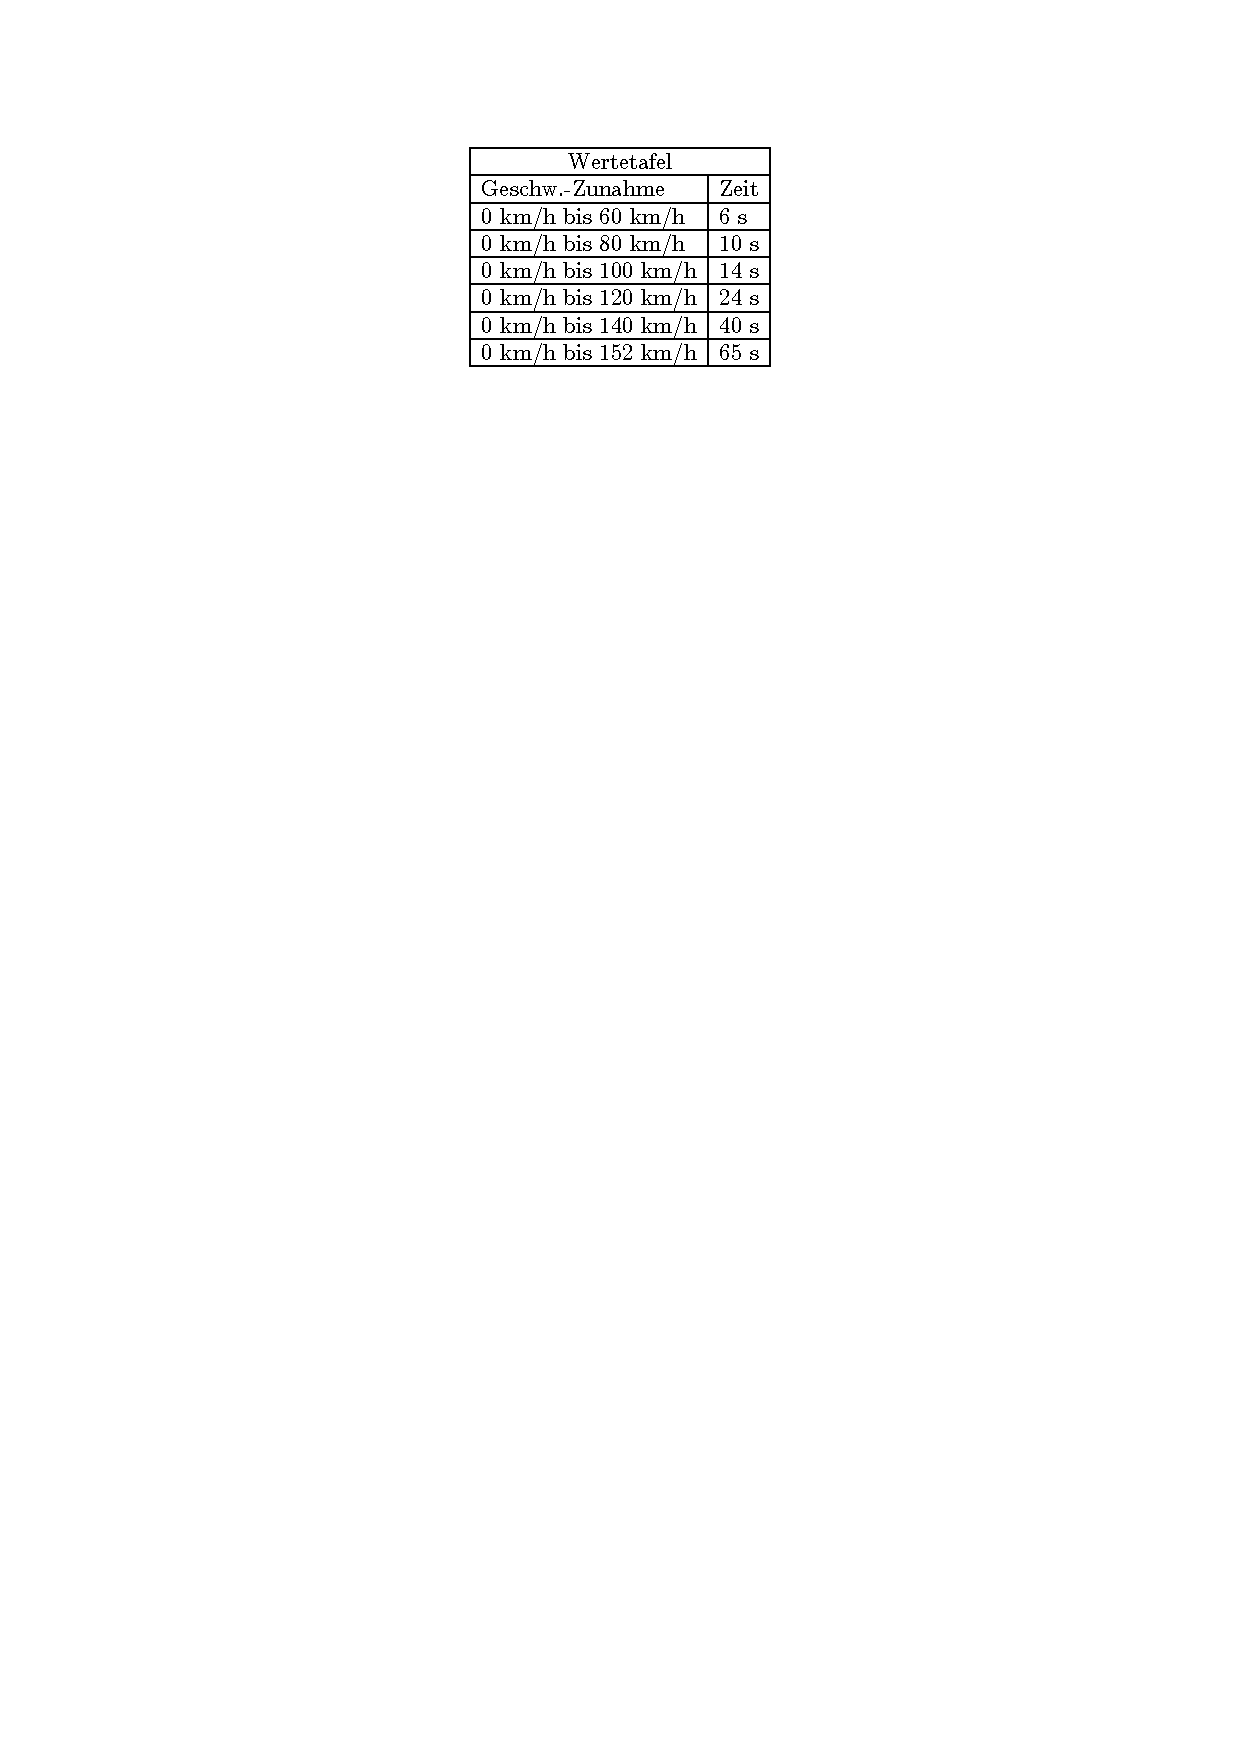
\includegraphics[width=\textwidth]{BilderKap1/Word-Tabelle-01.pdf}
\caption{Beispiel f�r eine MS-Word-Tabelle (kein Unterschied erkennbar).}
\label{bspmswordtabelle}
\end{center}
\end{table}

\textcolor{darkred}{Anzumerken ist noch, dass diese Tabelle felsenfest verankert wurde mit der Option [H] unter gleichzeitiger Verwendung des Packages float. Diese Ma�nahme ist nur bei sehr vielen, ungeplant wandernden Bildern oder ganz am Ende der Dokumentenerstellung sinnvoll, da sie sonst zu sehr in den Satz von Latex eingreift und unsch�ne L�cken entstehen l�sst.}


\clearpage

\textcolor{darkred}{Die nachfolgenden exemplarischen Vektorgrafiken wurden ebenfalls mit MS Word bzw. (fast gleichbedeutend) mit MS Visio erstellt und �ber pdf-Export und Zuschnitt mittels Adobe Acrobat (Beschneidungswerkzeug) im Latex-Dokument eingebettet.}

\textcolor{darkred}{Diese Art der Erstellung von Zeichnungsobjekten er�ffnet auch die M�glichkeit, Zeichnungen, Charts, CADs, UML-Diagramme o.�. mit jedwegem Programm zu erstellen, welches eine Druckoption bietet. Der Export geschieht dann �ber den Druckertreiber \glqq Adobe PDF\grqq\ (Vorsicht, dieser wird nur bei Vollinstallation des kommerziellen Adobe Acrobat-Studios installiert).}

\begin{figure}[htbp]
\centering
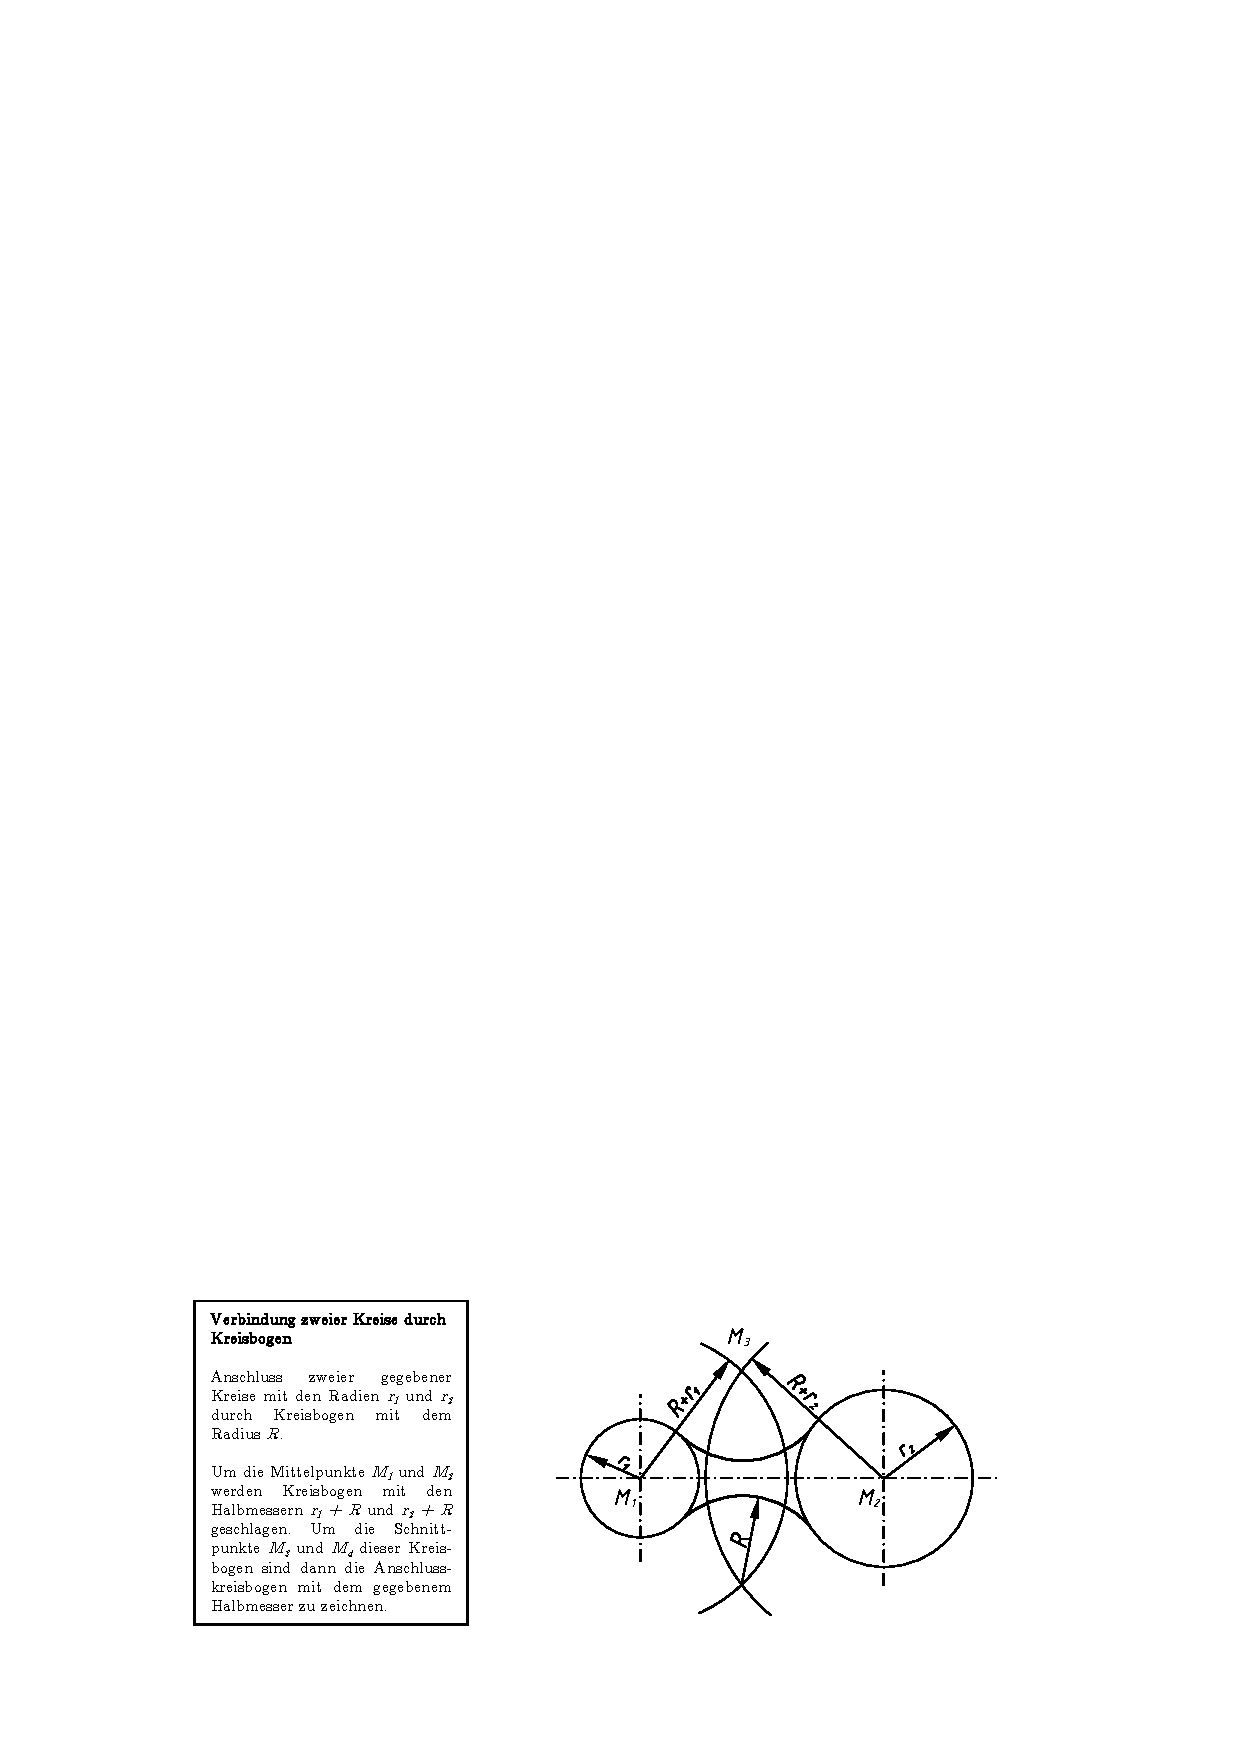
\includegraphics[width=0.99\textwidth]
{BilderKap1/Zeichenbeispiel-01.pdf}
\caption{Beispiel f�r eine Vektorgrafik (Fonts: DCR10, ISOCTEURItalic), Bildquelle: [Hoischen 88].}
\label{bspvektorgrafik}
\end{figure}

\textcolor{darkred}{Im zugeh�rigen Word-Dokument finden sich noch weitere Zeichnungen und Erkl�rungen, wie diese erstellt wurden. Weiterhin sind dort auch die zugeh�rigen Fonts abgelegt, welche f�r die Beispiele in das Verzeichnis \textbackslash windows\textbackslash fonts kopiert werden m�ssen.}

\index{Vektorgrafik}
\begin{figure}[htbp]
\centering
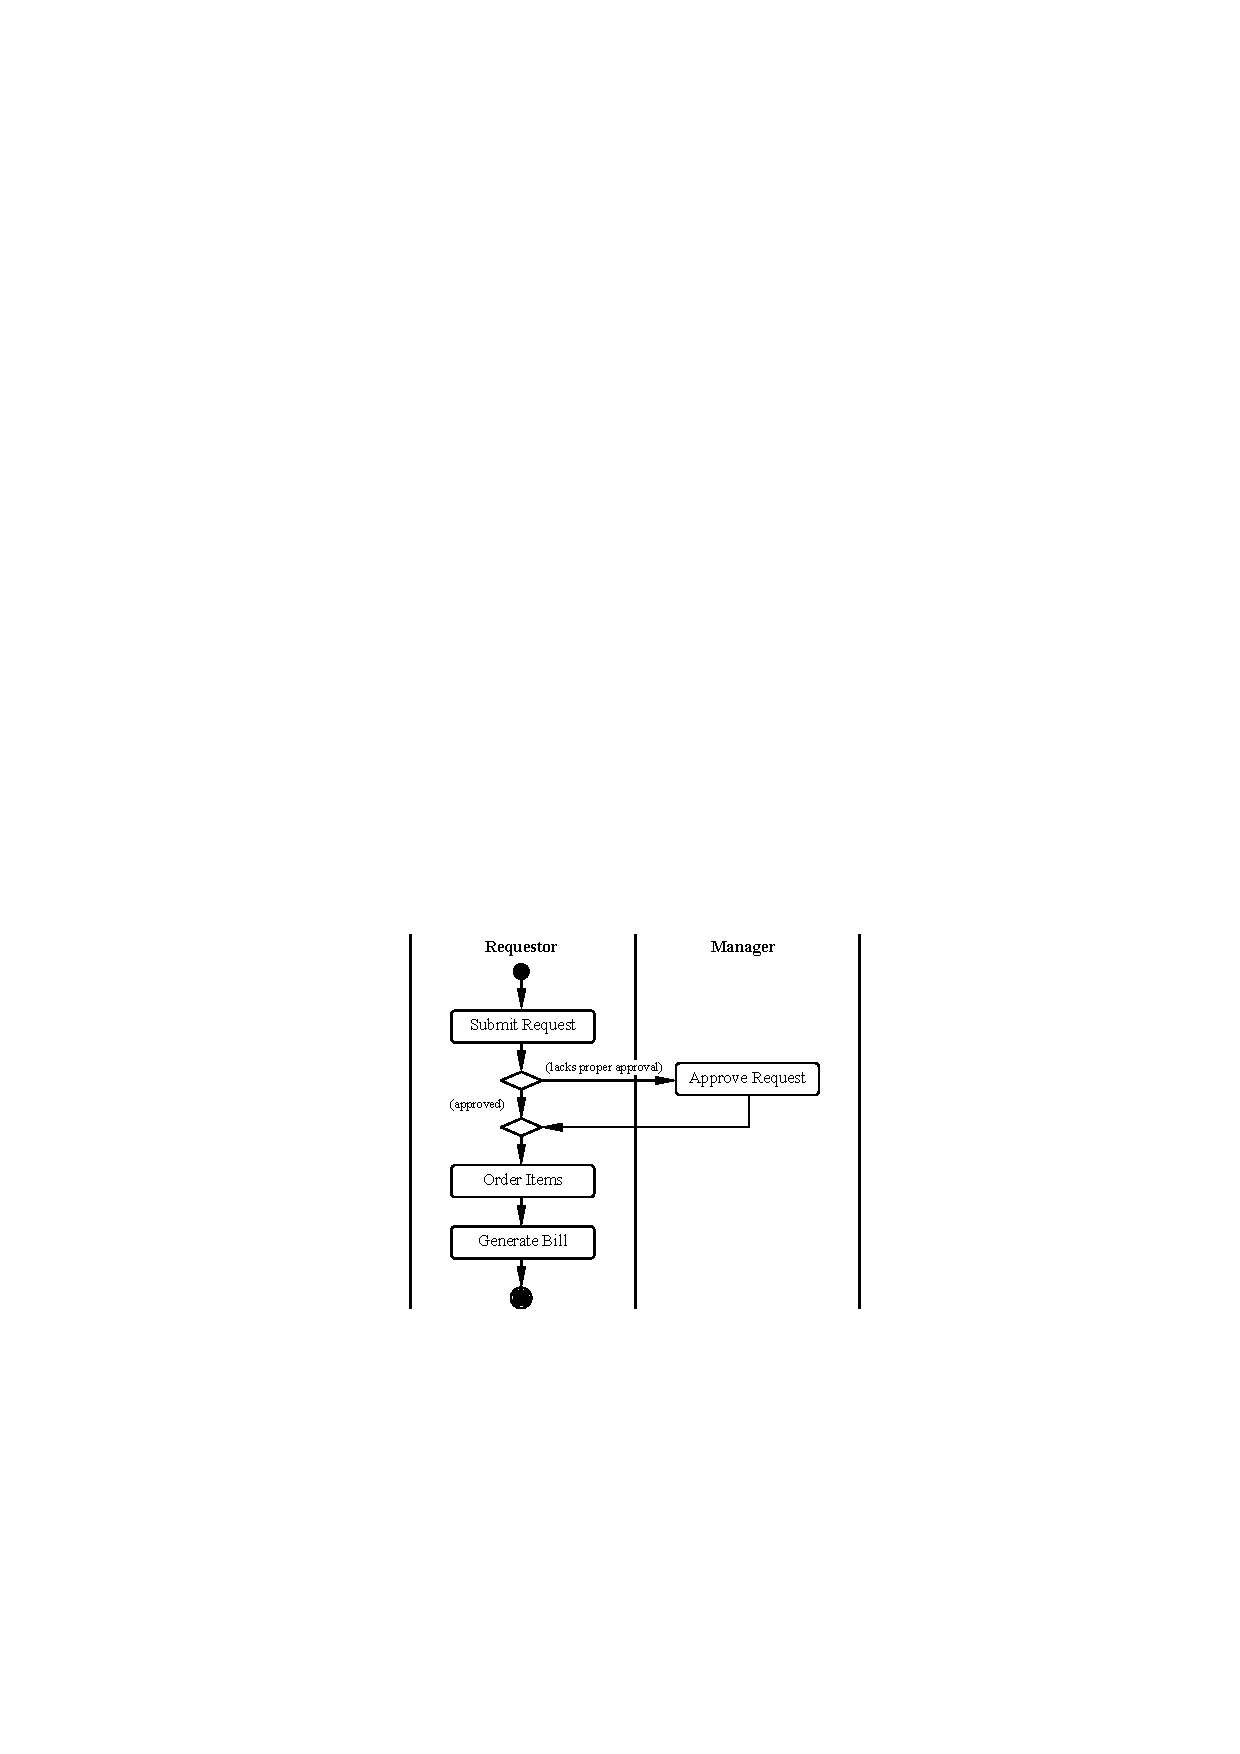
\includegraphics[width=0.99\textwidth]
{BilderKap1/Zeichenbeispiel-02.pdf}
\caption{Beispiel f�r eine Vektorgrafik (Font: Times New Roman).}
\label{bspvektorgrafik2}
\end{figure}


\clearpage
\index{Fonts}\index{Schrifteneinbettung}
\textcolor{darkred}{Beim Umgang mit .pdf-Dateien ist stets besonders darauf zu achten, dass die verwendeten Fonts eingebettet werden. Einstellbar ist dies im Adobe Acrobat �ber Bearbeiten / Grundeinstellungen / \dots . Eine Kontrolle erfolgt �ber Datei / Dokumenteigenschaften / Schriften oder �ber Erweitert / Preflight / Liste mit Text ohne eingebettete Schriften.}

\textcolor{darkred}{Verwenden Sie eine Version $\geq$ 6.0; gerade bei der Schrifteneinbettung gab es bei fr�heren Versionen �fters Schwierigkeiten.}



\medskip


%http://www.fnal.gov/docs/products/gnuplot/tutorial/
%http://gnuplot.sourceforge.net/docs/tutorial.pdf

\index{Gnuplot}
\begin {figure}[H]
\centering
% GNUPLOT: LaTeX picture
\setlength{\unitlength}{0.240900pt}
\ifx\plotpoint\undefined\newsavebox{\plotpoint}\fi
\begin{picture}(1500,900)(0,0)
\sbox{\plotpoint}{\rule[-0.200pt]{0.400pt}{0.400pt}}%
\put(221.0,123.0){\rule[-0.200pt]{4.818pt}{0.400pt}}
\put(201,123){\makebox(0,0)[r]{$-1$}}
\put(1419.0,123.0){\rule[-0.200pt]{4.818pt}{0.400pt}}
\put(221.0,287.0){\rule[-0.200pt]{4.818pt}{0.400pt}}
\put(201,287){\makebox(0,0)[r]{$-0.5$}}
\put(1419.0,287.0){\rule[-0.200pt]{4.818pt}{0.400pt}}
\put(221.0,450.0){\rule[-0.200pt]{4.818pt}{0.400pt}}
\put(201,450){\makebox(0,0)[r]{$0$}}
\put(1419.0,450.0){\rule[-0.200pt]{4.818pt}{0.400pt}}
\put(221.0,614.0){\rule[-0.200pt]{4.818pt}{0.400pt}}
\put(201,614){\makebox(0,0)[r]{$0.5$}}
\put(1419.0,614.0){\rule[-0.200pt]{4.818pt}{0.400pt}}
\put(221.0,777.0){\rule[-0.200pt]{4.818pt}{0.400pt}}
\put(201,777){\makebox(0,0)[r]{$1$}}
\put(1419.0,777.0){\rule[-0.200pt]{4.818pt}{0.400pt}}
\put(221.0,123.0){\rule[-0.200pt]{0.400pt}{4.818pt}}
\put(221,82){\makebox(0,0){$0$}}
\put(221.0,757.0){\rule[-0.200pt]{0.400pt}{4.818pt}}
\put(415.0,123.0){\rule[-0.200pt]{0.400pt}{4.818pt}}
\put(415,82){\makebox(0,0){$1$}}
\put(415.0,757.0){\rule[-0.200pt]{0.400pt}{4.818pt}}
\put(609.0,123.0){\rule[-0.200pt]{0.400pt}{4.818pt}}
\put(609,82){\makebox(0,0){$2$}}
\put(609.0,757.0){\rule[-0.200pt]{0.400pt}{4.818pt}}
\put(803.0,123.0){\rule[-0.200pt]{0.400pt}{4.818pt}}
\put(803,82){\makebox(0,0){$3$}}
\put(803.0,757.0){\rule[-0.200pt]{0.400pt}{4.818pt}}
\put(997.0,123.0){\rule[-0.200pt]{0.400pt}{4.818pt}}
\put(997,82){\makebox(0,0){$4$}}
\put(997.0,757.0){\rule[-0.200pt]{0.400pt}{4.818pt}}
\put(1191.0,123.0){\rule[-0.200pt]{0.400pt}{4.818pt}}
\put(1191,82){\makebox(0,0){$5$}}
\put(1191.0,757.0){\rule[-0.200pt]{0.400pt}{4.818pt}}
\put(1385.0,123.0){\rule[-0.200pt]{0.400pt}{4.818pt}}
\put(1385,82){\makebox(0,0){$6$}}
\put(1385.0,757.0){\rule[-0.200pt]{0.400pt}{4.818pt}}
\put(221.0,123.0){\rule[-0.200pt]{0.400pt}{157.549pt}}
\put(221.0,123.0){\rule[-0.200pt]{293.416pt}{0.400pt}}
\put(1439.0,123.0){\rule[-0.200pt]{0.400pt}{157.549pt}}
\put(221.0,777.0){\rule[-0.200pt]{293.416pt}{0.400pt}}
\put(40,450){\makebox(0,0){$y$-Achse}}
\put(830,21){\makebox(0,0){$x$-Achse}}
\put(830,839){\makebox(0,0){Ein Plot der Funktion $y=\sin(x)$}}
\put(1279,737){\makebox(0,0)[r]{sin(x)}}
\put(1299.0,737.0){\rule[-0.200pt]{24.090pt}{0.400pt}}
\put(221,450){\usebox{\plotpoint}}
\multiput(221.58,450.00)(0.492,0.884){21}{\rule{0.119pt}{0.800pt}}
\multiput(220.17,450.00)(12.000,19.340){2}{\rule{0.400pt}{0.400pt}}
\multiput(233.58,471.00)(0.493,0.774){23}{\rule{0.119pt}{0.715pt}}
\multiput(232.17,471.00)(13.000,18.515){2}{\rule{0.400pt}{0.358pt}}
\multiput(246.58,491.00)(0.492,0.884){21}{\rule{0.119pt}{0.800pt}}
\multiput(245.17,491.00)(12.000,19.340){2}{\rule{0.400pt}{0.400pt}}
\multiput(258.58,512.00)(0.492,0.841){21}{\rule{0.119pt}{0.767pt}}
\multiput(257.17,512.00)(12.000,18.409){2}{\rule{0.400pt}{0.383pt}}
\multiput(270.58,532.00)(0.493,0.774){23}{\rule{0.119pt}{0.715pt}}
\multiput(269.17,532.00)(13.000,18.515){2}{\rule{0.400pt}{0.358pt}}
\multiput(283.58,552.00)(0.492,0.798){21}{\rule{0.119pt}{0.733pt}}
\multiput(282.17,552.00)(12.000,17.478){2}{\rule{0.400pt}{0.367pt}}
\multiput(295.58,571.00)(0.492,0.798){21}{\rule{0.119pt}{0.733pt}}
\multiput(294.17,571.00)(12.000,17.478){2}{\rule{0.400pt}{0.367pt}}
\multiput(307.58,590.00)(0.492,0.798){21}{\rule{0.119pt}{0.733pt}}
\multiput(306.17,590.00)(12.000,17.478){2}{\rule{0.400pt}{0.367pt}}
\multiput(319.58,609.00)(0.493,0.695){23}{\rule{0.119pt}{0.654pt}}
\multiput(318.17,609.00)(13.000,16.643){2}{\rule{0.400pt}{0.327pt}}
\multiput(332.58,627.00)(0.492,0.712){21}{\rule{0.119pt}{0.667pt}}
\multiput(331.17,627.00)(12.000,15.616){2}{\rule{0.400pt}{0.333pt}}
\multiput(344.58,644.00)(0.492,0.669){21}{\rule{0.119pt}{0.633pt}}
\multiput(343.17,644.00)(12.000,14.685){2}{\rule{0.400pt}{0.317pt}}
\multiput(356.58,660.00)(0.493,0.616){23}{\rule{0.119pt}{0.592pt}}
\multiput(355.17,660.00)(13.000,14.771){2}{\rule{0.400pt}{0.296pt}}
\multiput(369.58,676.00)(0.492,0.582){21}{\rule{0.119pt}{0.567pt}}
\multiput(368.17,676.00)(12.000,12.824){2}{\rule{0.400pt}{0.283pt}}
\multiput(381.58,690.00)(0.492,0.582){21}{\rule{0.119pt}{0.567pt}}
\multiput(380.17,690.00)(12.000,12.824){2}{\rule{0.400pt}{0.283pt}}
\multiput(393.00,704.58)(0.539,0.492){21}{\rule{0.533pt}{0.119pt}}
\multiput(393.00,703.17)(11.893,12.000){2}{\rule{0.267pt}{0.400pt}}
\multiput(406.00,716.58)(0.496,0.492){21}{\rule{0.500pt}{0.119pt}}
\multiput(406.00,715.17)(10.962,12.000){2}{\rule{0.250pt}{0.400pt}}
\multiput(418.00,728.58)(0.600,0.491){17}{\rule{0.580pt}{0.118pt}}
\multiput(418.00,727.17)(10.796,10.000){2}{\rule{0.290pt}{0.400pt}}
\multiput(430.00,738.59)(0.669,0.489){15}{\rule{0.633pt}{0.118pt}}
\multiput(430.00,737.17)(10.685,9.000){2}{\rule{0.317pt}{0.400pt}}
\multiput(442.00,747.59)(0.824,0.488){13}{\rule{0.750pt}{0.117pt}}
\multiput(442.00,746.17)(11.443,8.000){2}{\rule{0.375pt}{0.400pt}}
\multiput(455.00,755.59)(0.874,0.485){11}{\rule{0.786pt}{0.117pt}}
\multiput(455.00,754.17)(10.369,7.000){2}{\rule{0.393pt}{0.400pt}}
\multiput(467.00,762.59)(1.033,0.482){9}{\rule{0.900pt}{0.116pt}}
\multiput(467.00,761.17)(10.132,6.000){2}{\rule{0.450pt}{0.400pt}}
\multiput(479.00,768.60)(1.797,0.468){5}{\rule{1.400pt}{0.113pt}}
\multiput(479.00,767.17)(10.094,4.000){2}{\rule{0.700pt}{0.400pt}}
\multiput(492.00,772.61)(2.472,0.447){3}{\rule{1.700pt}{0.108pt}}
\multiput(492.00,771.17)(8.472,3.000){2}{\rule{0.850pt}{0.400pt}}
\put(504,775.17){\rule{2.500pt}{0.400pt}}
\multiput(504.00,774.17)(6.811,2.000){2}{\rule{1.250pt}{0.400pt}}
\put(529,775.67){\rule{2.891pt}{0.400pt}}
\multiput(529.00,776.17)(6.000,-1.000){2}{\rule{1.445pt}{0.400pt}}
\put(541,774.17){\rule{2.500pt}{0.400pt}}
\multiput(541.00,775.17)(6.811,-2.000){2}{\rule{1.250pt}{0.400pt}}
\multiput(553.00,772.94)(1.651,-0.468){5}{\rule{1.300pt}{0.113pt}}
\multiput(553.00,773.17)(9.302,-4.000){2}{\rule{0.650pt}{0.400pt}}
\multiput(565.00,768.93)(1.378,-0.477){7}{\rule{1.140pt}{0.115pt}}
\multiput(565.00,769.17)(10.634,-5.000){2}{\rule{0.570pt}{0.400pt}}
\multiput(578.00,763.93)(1.033,-0.482){9}{\rule{0.900pt}{0.116pt}}
\multiput(578.00,764.17)(10.132,-6.000){2}{\rule{0.450pt}{0.400pt}}
\multiput(590.00,757.93)(0.874,-0.485){11}{\rule{0.786pt}{0.117pt}}
\multiput(590.00,758.17)(10.369,-7.000){2}{\rule{0.393pt}{0.400pt}}
\multiput(602.00,750.93)(0.728,-0.489){15}{\rule{0.678pt}{0.118pt}}
\multiput(602.00,751.17)(11.593,-9.000){2}{\rule{0.339pt}{0.400pt}}
\multiput(615.00,741.92)(0.600,-0.491){17}{\rule{0.580pt}{0.118pt}}
\multiput(615.00,742.17)(10.796,-10.000){2}{\rule{0.290pt}{0.400pt}}
\multiput(627.00,731.92)(0.543,-0.492){19}{\rule{0.536pt}{0.118pt}}
\multiput(627.00,732.17)(10.887,-11.000){2}{\rule{0.268pt}{0.400pt}}
\multiput(639.00,720.92)(0.539,-0.492){21}{\rule{0.533pt}{0.119pt}}
\multiput(639.00,721.17)(11.893,-12.000){2}{\rule{0.267pt}{0.400pt}}
\multiput(652.58,707.79)(0.492,-0.539){21}{\rule{0.119pt}{0.533pt}}
\multiput(651.17,708.89)(12.000,-11.893){2}{\rule{0.400pt}{0.267pt}}
\multiput(664.58,694.65)(0.492,-0.582){21}{\rule{0.119pt}{0.567pt}}
\multiput(663.17,695.82)(12.000,-12.824){2}{\rule{0.400pt}{0.283pt}}
\multiput(676.58,680.67)(0.493,-0.576){23}{\rule{0.119pt}{0.562pt}}
\multiput(675.17,681.83)(13.000,-13.834){2}{\rule{0.400pt}{0.281pt}}
\multiput(689.58,665.37)(0.492,-0.669){21}{\rule{0.119pt}{0.633pt}}
\multiput(688.17,666.69)(12.000,-14.685){2}{\rule{0.400pt}{0.317pt}}
\multiput(701.58,649.37)(0.492,-0.669){21}{\rule{0.119pt}{0.633pt}}
\multiput(700.17,650.69)(12.000,-14.685){2}{\rule{0.400pt}{0.317pt}}
\multiput(713.58,633.09)(0.492,-0.755){21}{\rule{0.119pt}{0.700pt}}
\multiput(712.17,634.55)(12.000,-16.547){2}{\rule{0.400pt}{0.350pt}}
\multiput(725.58,615.29)(0.493,-0.695){23}{\rule{0.119pt}{0.654pt}}
\multiput(724.17,616.64)(13.000,-16.643){2}{\rule{0.400pt}{0.327pt}}
\multiput(738.58,597.09)(0.492,-0.755){21}{\rule{0.119pt}{0.700pt}}
\multiput(737.17,598.55)(12.000,-16.547){2}{\rule{0.400pt}{0.350pt}}
\multiput(750.58,578.82)(0.492,-0.841){21}{\rule{0.119pt}{0.767pt}}
\multiput(749.17,580.41)(12.000,-18.409){2}{\rule{0.400pt}{0.383pt}}
\multiput(762.58,559.16)(0.493,-0.734){23}{\rule{0.119pt}{0.685pt}}
\multiput(761.17,560.58)(13.000,-17.579){2}{\rule{0.400pt}{0.342pt}}
\multiput(775.58,539.82)(0.492,-0.841){21}{\rule{0.119pt}{0.767pt}}
\multiput(774.17,541.41)(12.000,-18.409){2}{\rule{0.400pt}{0.383pt}}
\multiput(787.58,519.68)(0.492,-0.884){21}{\rule{0.119pt}{0.800pt}}
\multiput(786.17,521.34)(12.000,-19.340){2}{\rule{0.400pt}{0.400pt}}
\multiput(799.58,499.03)(0.493,-0.774){23}{\rule{0.119pt}{0.715pt}}
\multiput(798.17,500.52)(13.000,-18.515){2}{\rule{0.400pt}{0.358pt}}
\multiput(812.58,478.68)(0.492,-0.884){21}{\rule{0.119pt}{0.800pt}}
\multiput(811.17,480.34)(12.000,-19.340){2}{\rule{0.400pt}{0.400pt}}
\multiput(824.58,457.68)(0.492,-0.884){21}{\rule{0.119pt}{0.800pt}}
\multiput(823.17,459.34)(12.000,-19.340){2}{\rule{0.400pt}{0.400pt}}
\multiput(836.58,436.68)(0.492,-0.884){21}{\rule{0.119pt}{0.800pt}}
\multiput(835.17,438.34)(12.000,-19.340){2}{\rule{0.400pt}{0.400pt}}
\multiput(848.58,416.03)(0.493,-0.774){23}{\rule{0.119pt}{0.715pt}}
\multiput(847.17,417.52)(13.000,-18.515){2}{\rule{0.400pt}{0.358pt}}
\multiput(861.58,395.82)(0.492,-0.841){21}{\rule{0.119pt}{0.767pt}}
\multiput(860.17,397.41)(12.000,-18.409){2}{\rule{0.400pt}{0.383pt}}
\multiput(873.58,375.68)(0.492,-0.884){21}{\rule{0.119pt}{0.800pt}}
\multiput(872.17,377.34)(12.000,-19.340){2}{\rule{0.400pt}{0.400pt}}
\multiput(885.58,355.16)(0.493,-0.734){23}{\rule{0.119pt}{0.685pt}}
\multiput(884.17,356.58)(13.000,-17.579){2}{\rule{0.400pt}{0.342pt}}
\multiput(898.58,335.82)(0.492,-0.841){21}{\rule{0.119pt}{0.767pt}}
\multiput(897.17,337.41)(12.000,-18.409){2}{\rule{0.400pt}{0.383pt}}
\multiput(910.58,316.09)(0.492,-0.755){21}{\rule{0.119pt}{0.700pt}}
\multiput(909.17,317.55)(12.000,-16.547){2}{\rule{0.400pt}{0.350pt}}
\multiput(922.58,298.29)(0.493,-0.695){23}{\rule{0.119pt}{0.654pt}}
\multiput(921.17,299.64)(13.000,-16.643){2}{\rule{0.400pt}{0.327pt}}
\multiput(935.58,280.09)(0.492,-0.755){21}{\rule{0.119pt}{0.700pt}}
\multiput(934.17,281.55)(12.000,-16.547){2}{\rule{0.400pt}{0.350pt}}
\multiput(947.58,262.23)(0.492,-0.712){21}{\rule{0.119pt}{0.667pt}}
\multiput(946.17,263.62)(12.000,-15.616){2}{\rule{0.400pt}{0.333pt}}
\multiput(959.58,245.37)(0.492,-0.669){21}{\rule{0.119pt}{0.633pt}}
\multiput(958.17,246.69)(12.000,-14.685){2}{\rule{0.400pt}{0.317pt}}
\multiput(971.58,229.67)(0.493,-0.576){23}{\rule{0.119pt}{0.562pt}}
\multiput(970.17,230.83)(13.000,-13.834){2}{\rule{0.400pt}{0.281pt}}
\multiput(984.58,214.65)(0.492,-0.582){21}{\rule{0.119pt}{0.567pt}}
\multiput(983.17,215.82)(12.000,-12.824){2}{\rule{0.400pt}{0.283pt}}
\multiput(996.58,200.79)(0.492,-0.539){21}{\rule{0.119pt}{0.533pt}}
\multiput(995.17,201.89)(12.000,-11.893){2}{\rule{0.400pt}{0.267pt}}
\multiput(1008.00,188.92)(0.539,-0.492){21}{\rule{0.533pt}{0.119pt}}
\multiput(1008.00,189.17)(11.893,-12.000){2}{\rule{0.267pt}{0.400pt}}
\multiput(1021.00,176.92)(0.543,-0.492){19}{\rule{0.536pt}{0.118pt}}
\multiput(1021.00,177.17)(10.887,-11.000){2}{\rule{0.268pt}{0.400pt}}
\multiput(1033.00,165.92)(0.600,-0.491){17}{\rule{0.580pt}{0.118pt}}
\multiput(1033.00,166.17)(10.796,-10.000){2}{\rule{0.290pt}{0.400pt}}
\multiput(1045.00,155.93)(0.824,-0.488){13}{\rule{0.750pt}{0.117pt}}
\multiput(1045.00,156.17)(11.443,-8.000){2}{\rule{0.375pt}{0.400pt}}
\multiput(1058.00,147.93)(0.758,-0.488){13}{\rule{0.700pt}{0.117pt}}
\multiput(1058.00,148.17)(10.547,-8.000){2}{\rule{0.350pt}{0.400pt}}
\multiput(1070.00,139.93)(1.033,-0.482){9}{\rule{0.900pt}{0.116pt}}
\multiput(1070.00,140.17)(10.132,-6.000){2}{\rule{0.450pt}{0.400pt}}
\multiput(1082.00,133.93)(1.378,-0.477){7}{\rule{1.140pt}{0.115pt}}
\multiput(1082.00,134.17)(10.634,-5.000){2}{\rule{0.570pt}{0.400pt}}
\multiput(1095.00,128.94)(1.651,-0.468){5}{\rule{1.300pt}{0.113pt}}
\multiput(1095.00,129.17)(9.302,-4.000){2}{\rule{0.650pt}{0.400pt}}
\put(1107,124.17){\rule{2.500pt}{0.400pt}}
\multiput(1107.00,125.17)(6.811,-2.000){2}{\rule{1.250pt}{0.400pt}}
\put(1119,122.67){\rule{2.891pt}{0.400pt}}
\multiput(1119.00,123.17)(6.000,-1.000){2}{\rule{1.445pt}{0.400pt}}
\put(516.0,777.0){\rule[-0.200pt]{3.132pt}{0.400pt}}
\put(1144,123.17){\rule{2.500pt}{0.400pt}}
\multiput(1144.00,122.17)(6.811,2.000){2}{\rule{1.250pt}{0.400pt}}
\multiput(1156.00,125.61)(2.472,0.447){3}{\rule{1.700pt}{0.108pt}}
\multiput(1156.00,124.17)(8.472,3.000){2}{\rule{0.850pt}{0.400pt}}
\multiput(1168.00,128.60)(1.797,0.468){5}{\rule{1.400pt}{0.113pt}}
\multiput(1168.00,127.17)(10.094,4.000){2}{\rule{0.700pt}{0.400pt}}
\multiput(1181.00,132.59)(1.033,0.482){9}{\rule{0.900pt}{0.116pt}}
\multiput(1181.00,131.17)(10.132,6.000){2}{\rule{0.450pt}{0.400pt}}
\multiput(1193.00,138.59)(1.033,0.482){9}{\rule{0.900pt}{0.116pt}}
\multiput(1193.00,137.17)(10.132,6.000){2}{\rule{0.450pt}{0.400pt}}
\multiput(1205.00,144.59)(0.824,0.488){13}{\rule{0.750pt}{0.117pt}}
\multiput(1205.00,143.17)(11.443,8.000){2}{\rule{0.375pt}{0.400pt}}
\multiput(1218.00,152.59)(0.669,0.489){15}{\rule{0.633pt}{0.118pt}}
\multiput(1218.00,151.17)(10.685,9.000){2}{\rule{0.317pt}{0.400pt}}
\multiput(1230.00,161.58)(0.543,0.492){19}{\rule{0.536pt}{0.118pt}}
\multiput(1230.00,160.17)(10.887,11.000){2}{\rule{0.268pt}{0.400pt}}
\multiput(1242.00,172.58)(0.543,0.492){19}{\rule{0.536pt}{0.118pt}}
\multiput(1242.00,171.17)(10.887,11.000){2}{\rule{0.268pt}{0.400pt}}
\multiput(1254.00,183.58)(0.497,0.493){23}{\rule{0.500pt}{0.119pt}}
\multiput(1254.00,182.17)(11.962,13.000){2}{\rule{0.250pt}{0.400pt}}
\multiput(1267.58,196.00)(0.492,0.539){21}{\rule{0.119pt}{0.533pt}}
\multiput(1266.17,196.00)(12.000,11.893){2}{\rule{0.400pt}{0.267pt}}
\multiput(1279.58,209.00)(0.492,0.625){21}{\rule{0.119pt}{0.600pt}}
\multiput(1278.17,209.00)(12.000,13.755){2}{\rule{0.400pt}{0.300pt}}
\multiput(1291.58,224.00)(0.493,0.576){23}{\rule{0.119pt}{0.562pt}}
\multiput(1290.17,224.00)(13.000,13.834){2}{\rule{0.400pt}{0.281pt}}
\multiput(1304.58,239.00)(0.492,0.669){21}{\rule{0.119pt}{0.633pt}}
\multiput(1303.17,239.00)(12.000,14.685){2}{\rule{0.400pt}{0.317pt}}
\multiput(1316.58,255.00)(0.492,0.712){21}{\rule{0.119pt}{0.667pt}}
\multiput(1315.17,255.00)(12.000,15.616){2}{\rule{0.400pt}{0.333pt}}
\multiput(1328.58,272.00)(0.493,0.695){23}{\rule{0.119pt}{0.654pt}}
\multiput(1327.17,272.00)(13.000,16.643){2}{\rule{0.400pt}{0.327pt}}
\multiput(1341.58,290.00)(0.492,0.798){21}{\rule{0.119pt}{0.733pt}}
\multiput(1340.17,290.00)(12.000,17.478){2}{\rule{0.400pt}{0.367pt}}
\multiput(1353.58,309.00)(0.492,0.798){21}{\rule{0.119pt}{0.733pt}}
\multiput(1352.17,309.00)(12.000,17.478){2}{\rule{0.400pt}{0.367pt}}
\multiput(1365.58,328.00)(0.492,0.798){21}{\rule{0.119pt}{0.733pt}}
\multiput(1364.17,328.00)(12.000,17.478){2}{\rule{0.400pt}{0.367pt}}
\multiput(1377.58,347.00)(0.493,0.774){23}{\rule{0.119pt}{0.715pt}}
\multiput(1376.17,347.00)(13.000,18.515){2}{\rule{0.400pt}{0.358pt}}
\multiput(1390.58,367.00)(0.492,0.841){21}{\rule{0.119pt}{0.767pt}}
\multiput(1389.17,367.00)(12.000,18.409){2}{\rule{0.400pt}{0.383pt}}
\multiput(1402.58,387.00)(0.492,0.884){21}{\rule{0.119pt}{0.800pt}}
\multiput(1401.17,387.00)(12.000,19.340){2}{\rule{0.400pt}{0.400pt}}
\multiput(1414.58,408.00)(0.493,0.774){23}{\rule{0.119pt}{0.715pt}}
\multiput(1413.17,408.00)(13.000,18.515){2}{\rule{0.400pt}{0.358pt}}
\multiput(1427.58,428.00)(0.492,0.884){21}{\rule{0.119pt}{0.800pt}}
\multiput(1426.17,428.00)(12.000,19.340){2}{\rule{0.400pt}{0.400pt}}
\put(1131.0,123.0){\rule[-0.200pt]{3.132pt}{0.400pt}}
\put(221.0,123.0){\rule[-0.200pt]{0.400pt}{157.549pt}}
\put(221.0,123.0){\rule[-0.200pt]{293.416pt}{0.400pt}}
\put(1439.0,123.0){\rule[-0.200pt]{0.400pt}{157.549pt}}
\put(221.0,777.0){\rule[-0.200pt]{293.416pt}{0.400pt}}
\end{picture}

\caption{Beispiel f�r eine Gnuplot-Kurve.}
\end {figure}



\begin {figure}[H]
\centering
% GNUPLOT: LaTeX picture
\setlength{\unitlength}{0.240900pt}
\ifx\plotpoint\undefined\newsavebox{\plotpoint}\fi
\begin{picture}(1500,900)(0,0)
\sbox{\plotpoint}{\rule[-0.200pt]{0.400pt}{0.400pt}}%
\put(221.0,123.0){\rule[-0.200pt]{4.818pt}{0.400pt}}
\put(201,123){\makebox(0,0)[r]{$0.2$}}
\put(1419.0,123.0){\rule[-0.200pt]{4.818pt}{0.400pt}}
\put(221.0,205.0){\rule[-0.200pt]{4.818pt}{0.400pt}}
\put(201,205){\makebox(0,0)[r]{$0.25$}}
\put(1419.0,205.0){\rule[-0.200pt]{4.818pt}{0.400pt}}
\put(221.0,286.0){\rule[-0.200pt]{4.818pt}{0.400pt}}
\put(201,286){\makebox(0,0)[r]{$0.3$}}
\put(1419.0,286.0){\rule[-0.200pt]{4.818pt}{0.400pt}}
\put(221.0,368.0){\rule[-0.200pt]{4.818pt}{0.400pt}}
\put(201,368){\makebox(0,0)[r]{$0.35$}}
\put(1419.0,368.0){\rule[-0.200pt]{4.818pt}{0.400pt}}
\put(221.0,450.0){\rule[-0.200pt]{4.818pt}{0.400pt}}
\put(201,450){\makebox(0,0)[r]{$0.4$}}
\put(1419.0,450.0){\rule[-0.200pt]{4.818pt}{0.400pt}}
\put(221.0,532.0){\rule[-0.200pt]{4.818pt}{0.400pt}}
\put(201,532){\makebox(0,0)[r]{$0.45$}}
\put(1419.0,532.0){\rule[-0.200pt]{4.818pt}{0.400pt}}
\put(221.0,613.0){\rule[-0.200pt]{4.818pt}{0.400pt}}
\put(201,613){\makebox(0,0)[r]{$0.5$}}
\put(1419.0,613.0){\rule[-0.200pt]{4.818pt}{0.400pt}}
\put(221.0,695.0){\rule[-0.200pt]{4.818pt}{0.400pt}}
\put(201,695){\makebox(0,0)[r]{$0.55$}}
\put(1419.0,695.0){\rule[-0.200pt]{4.818pt}{0.400pt}}
\put(221.0,777.0){\rule[-0.200pt]{4.818pt}{0.400pt}}
\put(201,777){\makebox(0,0)[r]{$0.6$}}
\put(1419.0,777.0){\rule[-0.200pt]{4.818pt}{0.400pt}}
\put(221.0,123.0){\rule[-0.200pt]{0.400pt}{4.818pt}}
\put(221,82){\makebox(0,0){$0$}}
\put(221.0,757.0){\rule[-0.200pt]{0.400pt}{4.818pt}}
\put(395.0,123.0){\rule[-0.200pt]{0.400pt}{4.818pt}}
\put(395,82){\makebox(0,0){$20$}}
\put(395.0,757.0){\rule[-0.200pt]{0.400pt}{4.818pt}}
\put(569.0,123.0){\rule[-0.200pt]{0.400pt}{4.818pt}}
\put(569,82){\makebox(0,0){$40$}}
\put(569.0,757.0){\rule[-0.200pt]{0.400pt}{4.818pt}}
\put(743.0,123.0){\rule[-0.200pt]{0.400pt}{4.818pt}}
\put(743,82){\makebox(0,0){$60$}}
\put(743.0,757.0){\rule[-0.200pt]{0.400pt}{4.818pt}}
\put(917.0,123.0){\rule[-0.200pt]{0.400pt}{4.818pt}}
\put(917,82){\makebox(0,0){$80$}}
\put(917.0,757.0){\rule[-0.200pt]{0.400pt}{4.818pt}}
\put(1091.0,123.0){\rule[-0.200pt]{0.400pt}{4.818pt}}
\put(1091,82){\makebox(0,0){$100$}}
\put(1091.0,757.0){\rule[-0.200pt]{0.400pt}{4.818pt}}
\put(1265.0,123.0){\rule[-0.200pt]{0.400pt}{4.818pt}}
\put(1265,82){\makebox(0,0){$120$}}
\put(1265.0,757.0){\rule[-0.200pt]{0.400pt}{4.818pt}}
\put(1439.0,123.0){\rule[-0.200pt]{0.400pt}{4.818pt}}
\put(1439,82){\makebox(0,0){$140$}}
\put(1439.0,757.0){\rule[-0.200pt]{0.400pt}{4.818pt}}
\put(221.0,123.0){\rule[-0.200pt]{0.400pt}{157.549pt}}
\put(221.0,123.0){\rule[-0.200pt]{293.416pt}{0.400pt}}
\put(1439.0,123.0){\rule[-0.200pt]{0.400pt}{157.549pt}}
\put(221.0,777.0){\rule[-0.200pt]{293.416pt}{0.400pt}}
\put(40,450){\makebox(0,0){$U$/V}}
\put(830,21){\makebox(0,0){$t$/s}}
\put(830,839){\makebox(0,0){Varianz des Messwertes}}
\put(1279,737){\makebox(0,0)[r]{'Beispieldaten-02.txt'}}
\put(1299.0,737.0){\rule[-0.200pt]{24.090pt}{0.400pt}}
\put(221,427){\usebox{\plotpoint}}
\multiput(221.00,425.92)(1.181,-0.498){71}{\rule{1.041pt}{0.120pt}}
\multiput(221.00,426.17)(84.840,-37.000){2}{\rule{0.520pt}{0.400pt}}
\multiput(308.00,388.93)(7.814,-0.482){9}{\rule{5.900pt}{0.116pt}}
\multiput(308.00,389.17)(74.754,-6.000){2}{\rule{2.950pt}{0.400pt}}
\put(395,382.17){\rule{17.500pt}{0.400pt}}
\multiput(395.00,383.17)(50.678,-2.000){2}{\rule{8.750pt}{0.400pt}}
\multiput(482.00,380.92)(0.670,-0.499){127}{\rule{0.635pt}{0.120pt}}
\multiput(482.00,381.17)(85.681,-65.000){2}{\rule{0.318pt}{0.400pt}}
\multiput(569.58,317.00)(0.499,2.375){171}{\rule{0.120pt}{1.994pt}}
\multiput(568.17,317.00)(87.000,407.861){2}{\rule{0.400pt}{0.997pt}}
\multiput(656.00,727.92)(2.000,-0.496){41}{\rule{1.682pt}{0.120pt}}
\multiput(656.00,728.17)(83.509,-22.000){2}{\rule{0.841pt}{0.400pt}}
\multiput(743.58,699.35)(0.499,-2.184){171}{\rule{0.120pt}{1.843pt}}
\multiput(742.17,703.18)(87.000,-375.176){2}{\rule{0.400pt}{0.921pt}}
\multiput(830.00,328.58)(0.702,0.499){121}{\rule{0.661pt}{0.120pt}}
\multiput(830.00,327.17)(85.627,62.000){2}{\rule{0.331pt}{0.400pt}}
\multiput(917.00,388.93)(7.814,-0.482){9}{\rule{5.900pt}{0.116pt}}
\multiput(917.00,389.17)(74.754,-6.000){2}{\rule{2.950pt}{0.400pt}}
\multiput(1004.58,381.68)(0.499,-0.575){171}{\rule{0.120pt}{0.560pt}}
\multiput(1003.17,382.84)(87.000,-98.838){2}{\rule{0.400pt}{0.280pt}}
\multiput(1091.58,284.00)(0.499,1.504){171}{\rule{0.120pt}{1.300pt}}
\multiput(1090.17,284.00)(87.000,258.302){2}{\rule{0.400pt}{0.650pt}}
\multiput(1178.58,541.44)(0.499,-0.950){171}{\rule{0.120pt}{0.859pt}}
\multiput(1177.17,543.22)(87.000,-163.218){2}{\rule{0.400pt}{0.429pt}}
\multiput(1265.58,375.20)(0.499,-1.325){171}{\rule{0.120pt}{1.157pt}}
\multiput(1264.17,377.60)(87.000,-227.598){2}{\rule{0.400pt}{0.579pt}}
\put(221.0,123.0){\rule[-0.200pt]{0.400pt}{157.549pt}}
\put(221.0,123.0){\rule[-0.200pt]{293.416pt}{0.400pt}}
\put(1439.0,123.0){\rule[-0.200pt]{0.400pt}{157.549pt}}
\put(221.0,777.0){\rule[-0.200pt]{293.416pt}{0.400pt}}
\end{picture}

\caption{Beispiel f�r einen Messwert-Plot mit Gnuplot.}
\end {figure}


\begin{figure}[H]
\centering
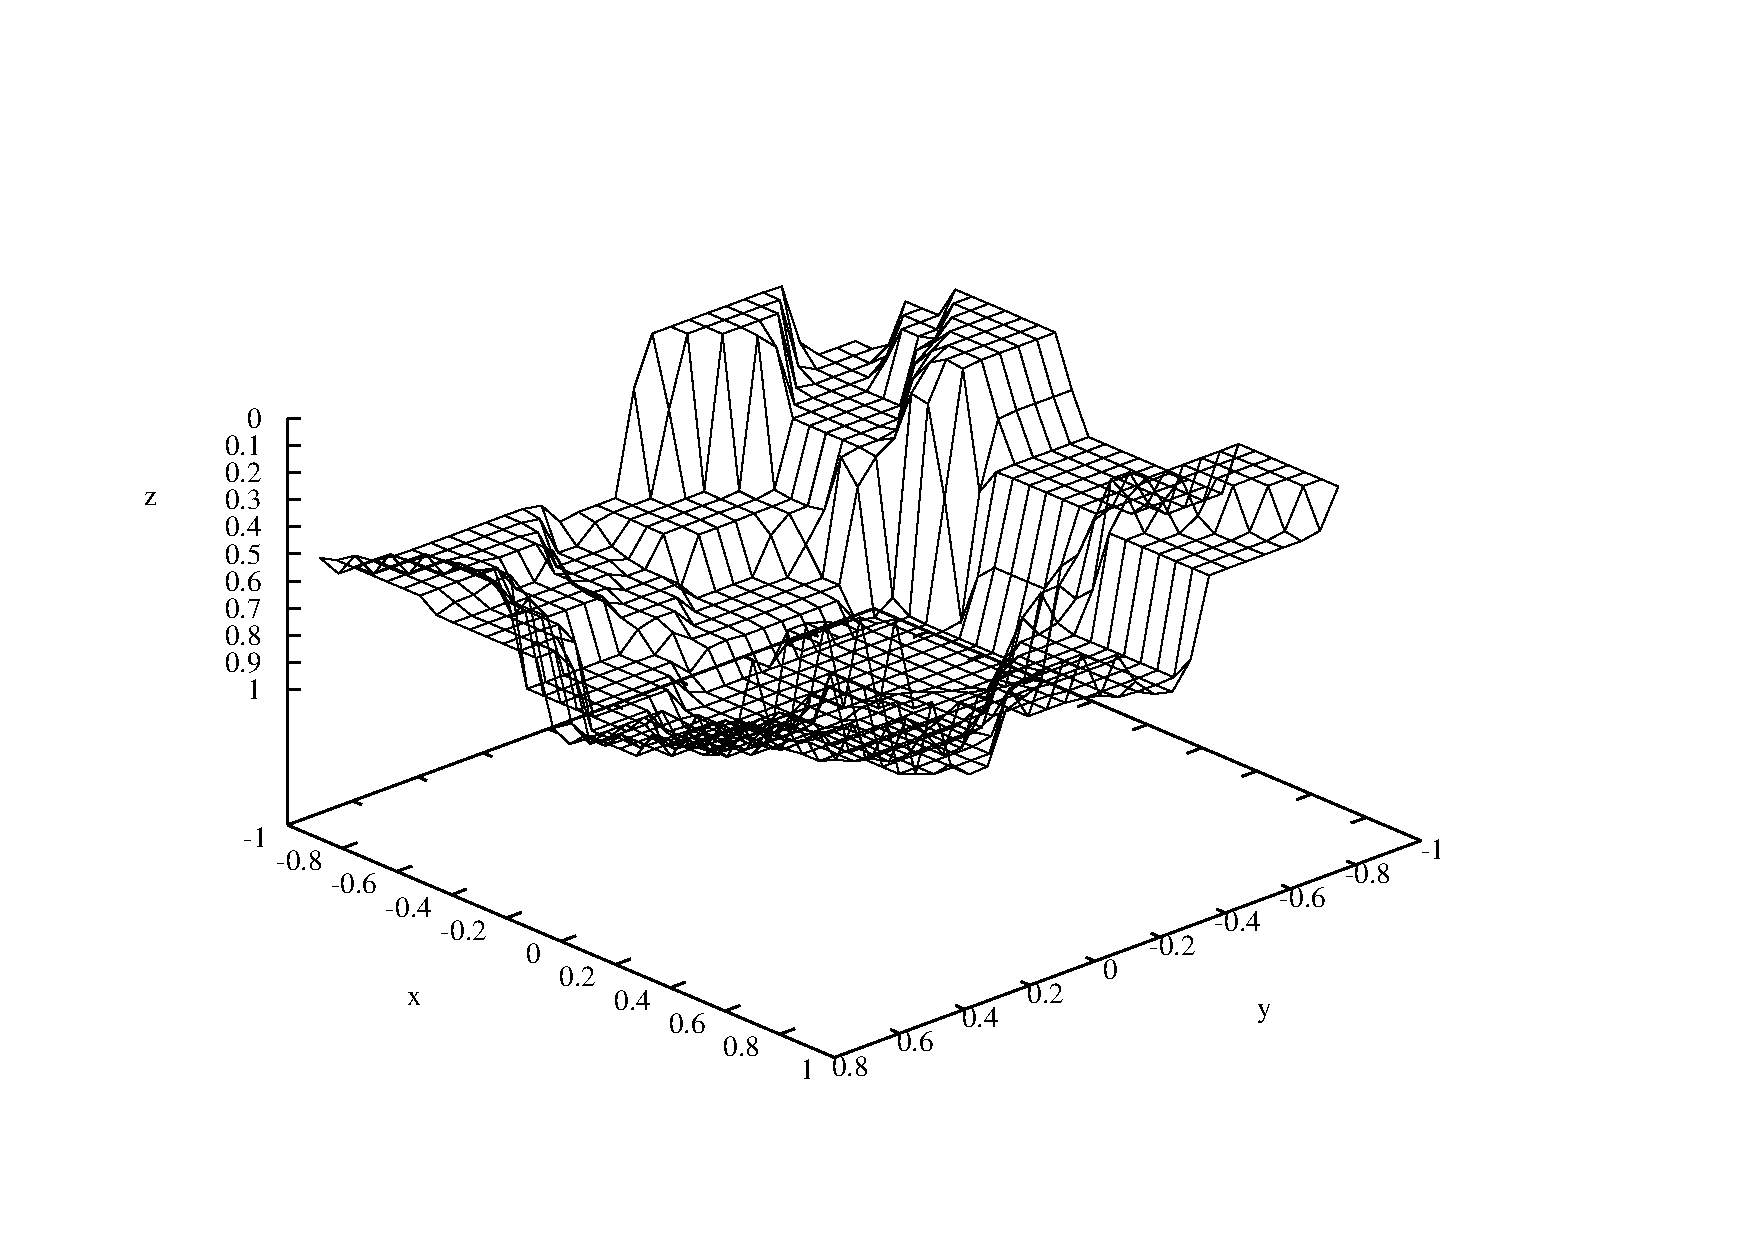
\includegraphics[width=0.90\textwidth]
{BilderKap1/gnuplot-03.pdf}
\caption{Beispiel f�r einen 3D-Plot mit Gnuplot (Ausgabe im Postscript-Format, dann Konvertierung nach pdf mittels Ghostscript).}
\label{bspgnuplot}
\end{figure}


Lorem ipsum dolor sit amet, consectetur adipisici elit, sed eiusmod tempor incidunt ut labore et dolore magna aliqua. Ut enim ad minim veniam, quis nostrud exercitation ullamco laboris nisi ut aliquid ex ea commodi consequat. Quis aute iure reprehenderit in voluptate velit esse cillum dolore eu fugiat nulla pariatur. Excepteur sint obcaecat cupiditat non proident, sunt in culpa qui officia deserunt mollit anim id est laborum.




\clearpage




\textcolor{darkred}{Einschub: Kommentare im Latex-Quelltext sind auf zwei Arten m�glich:}

\textcolor{darkred}{1.) Umwandlung einer Zeile bzw. eines zusammenh�ngenden Absatzes zum Kommentar: Durch ein vorangestelltes \%.}

\textcolor{darkred}{2.) Umwandlung eines l�ngeren Blocks zum Kommentar: Mittels Klammerung:}

\verb$\usepackage{verbatim}$\\
\verb$\begin{comment}$\\
\verb$    Dies ist ein Kommentar$\\
\verb$\end{comment}$\\


\textcolor{darkred}{Einschub: der Befehl \textbackslash verb\$\dots\$ erm�glicht die Eingabe eines Textes zwischen den Dollarzeichen, der nicht von Latex interpretiert wird. Somit stellt der Befehl die einfachste Art dar, Text mit vielen Sonderzeichen einzugeben. Typischerweise sind dies Quelltextzeilen, Dateinamen, Verzeichnisnamen, Programmaufrufe mit Parametern und URLs. Ausgegeben wird der Text in der Schriftart Courier New.}
\medskip

\textcolor{darkred}{Beispiel, ein Compiler-Aufruf:}\\
\verb$sdcc -I c:\sdcc\include -L c:\sdcc\lib\large simpletest.c --model-large$




\medskip
\textcolor{darkred}{Beispiel, mit angedeuteten Leerzeichen, einstellbar via \textbackslash verb*\$\dots\$:}\\
\verb*$sdcc -I c:\sdcc\include -L c:\sdcc\lib\large simpletest.c --model-large$




\medskip
\medskip
\medskip

\textcolor{darkred}{***}

\medskip

\textcolor{darkred}{Zu Formelsatz und Algorithmen: vgl. Anhang A: Mathematik.}



%

\chapter{Stand der Technik}



\section{Klassifizierung der Verfahren zur \dots}

Lorem ipsum dolor sit amet, consectetur adipisici elit, sed eiusmod tempor incidunt ut labore et dolore magna aliqua. Ut enim ad minim veniam, quis nostrud exercitation ullamco laboris nisi ut aliquid ex ea commodi consequat. Quis aute iure reprehenderit in voluptate velit esse cillum dolore eu fugiat nulla pariatur. Excepteur sint obcaecat cupiditat non proident, sunt in culpa qui officia deserunt mollit anim id est laborum.


\section{Vergleich und Bewertung der Verfahren}

Lorem ipsum dolor sit amet, consectetur adipisici elit, sed eiusmod tempor incidunt ut labore et dolore magna aliqua. Ut enim ad minim veniam, quis nostrud exercitation ullamco laboris nisi ut aliquid ex ea commodi consequat. Quis aute iure reprehenderit in voluptate velit esse cillum dolore eu fugiat nulla pariatur. Excepteur sint obcaecat cupiditat non proident, sunt in culpa qui officia deserunt mollit anim id est laborum.

Duis autem vel eum iriure dolor in hendrerit in vulputate velit esse molestie consequat, vel illum dolore eu feugiat nulla facilisis at vero eros et accumsan et iusto odio dignissim qui blandit praesent luptatum zzril delenit augue duis dolore te feugait nulla facilisi. Lorem ipsum dolor sit amet, consectetuer adipiscing elit, sed diam nonummy nibh euismod tincidunt ut laoreet dolore magna aliquam erat volutpat.

\chapter{Grundlagen}


\section{Text}
Lorem ipsum dolor sit amet, consectetur adipisici elit, sed eiusmod tempor incidunt ut labore et dolore magna aliqua. Ut enim ad minim veniam, quis nostrud exercitation ullamco laboris nisi ut aliquid ex ea commodi consequat. Quis aute iure reprehenderit in voluptate velit esse cillum dolore eu fugiat nulla pariatur. Excepteur sint obcaecat cupiditat non proident, sunt in culpa qui officia deserunt mollit anim id est laborum.

\section{Text}
Lorem ipsum dolor sit amet, consectetur adipisici elit, sed eiusmod tempor incidunt ut labore et dolore magna aliqua. Ut enim ad minim veniam, quis nostrud exercitation ullamco laboris nisi ut aliquid ex ea commodi consequat. Quis aute iure reprehenderit in voluptate velit esse cillum dolore eu fugiat nulla pariatur. Excepteur sint obcaecat cupiditat non proident, sunt in culpa qui officia deserunt mollit anim id est laborum.

\subsection{Text}
Lorem ipsum dolor sit amet, consectetur adipisici elit, sed eiusmod tempor incidunt ut labore et dolore magna aliqua. Ut enim ad minim veniam, quis nostrud exercitation ullamco laboris nisi ut aliquid ex ea commodi consequat. Quis aute iure reprehenderit in voluptate velit esse cillum dolore eu fugiat nulla pariatur. Excepteur sint obcaecat cupiditat non proident, sunt in culpa qui officia deserunt mollit anim id est laborum.

\subsection{Text}
Lorem ipsum dolor sit amet, consectetur adipisici elit, sed eiusmod tempor incidunt ut labore et dolore magna aliqua. Ut enim ad minim veniam, quis nostrud exercitation ullamco laboris nisi ut aliquid ex ea commodi consequat. Quis aute iure reprehenderit in voluptate velit esse cillum dolore eu
Lorem ipsum dolor sit amet, consectetur adipisici elit, sed eiusmod tempor incidunt ut labore et dolore magna aliqua. Ut enim ad minim veniam, quis nostrud exercitation ullamco laboris nisi ut aliquid ex ea commodi consequat. Quis aute iure reprehenderit in voluptate velit esse cillum dolore eu

\section{Text}
Lorem ipsum dolor sit amet, consectetur adipisici elit, sed eiusmod.nostrud exercitation ullamco laboris nisi ut aliquid ex ea commodi consequat. Quis aute iure reprehenderit in voluptate velit esse cillum dolore eu fugiat nulla pariatur. Excepteur sint obcaecat cupiditat non proident, sunt in culpa qui officia deserunt mollit anim id est laborum.










%







\chapter{Umsetzung}



\section{Text}
Lorem ipsum dolor sit amet, consectetur adipisici elit, sed eiusmod tempor incidunt ut labore et dolore magna aliqua. Ut enim ad minim veniam, quis nostrud exercitation ullamco laboris nisi ut aliquid ex ea commodi consequat. Quis aute iure reprehenderit in voluptate velit esse cillum dolore eu.

\section{Text}
Lorem ipsum dolor sit amet, consectetur adipisici elit, sed eiusmod tempor incidunt ut labore et dolore magna aliqua. Ut enim ad minim veniam, quis nostrud exercitation ullamco laboris nisi ut aliquid ex ea commodi consequat. Quis aute iure reprehenderit in voluptate velit esse cillum dolore eu fugiat nulla pariatur. Excepteur sint obcaecat cupiditat non proident, sunt in culpa qui officia deserunt mollit anim id est laborum. Duis autem vel.

\section{Text}
Lorem ipsum dolor sit amet, consectetur adipisici elit, sed eiusmod tempor incidunt ut labore et dolore magna aliqua. Ut enim ad minim veniam, quis nostrud exercitation ullamco laboris nisi ut aliquid ex ea commodi consequat. Quis aute iure reprehenderit in voluptate velit esse cillum dolore eu fugiat nulla pariatur. Excepteur sint obcaecat cupiditat non proident, sunt in culpa qui officia deserunt mollit anim id est laborum.

Lorem ipsum dolor sit amet, consectetur adipisici elit, sed eiusmod tempor incidunt ut labore et dolore magna aliqua. Ut enim ad minim veniam, quis nostrud exercitation ullamco laboris nisi ut aliquid ex ea commodi consequat. Quis aute iure reprehenderit in voluptate velit esse cillum dolore eu fugiat nulla pariatur. Excepteur sint obcaecat cupiditat non proident, sunt in culpa qui officia deserunt mollit anim id est laborum.



\chapter{Systemarchitektur}



\section{Hardware}
Lorem ipsum dolor sit amet, consectetur adipisici elit, sed eiusmod tempor incidunt ut labore et dolore magna aliqua. Ut enim ad minim veniam, quis nostrud exercitation ullamco.

\section{Software}
Lorem ipsum dolor sit amet, consectetur adipisici elit, sed eiusmod tempor incidunt ut labore et dolore magna aliqua. Ut enim ad minim veniam, quis nostrud exercitation ullamco.

\subsection{Verwendete Bibliotheken}
Duis autem vel eum iriure dolor in hendrerit in vulputate velit esse molestie consequat, vel illum dolore eu feugiat nulla facilisis at vero eros et accumsan et iusto odio dignissim qui.

\subsection{Klassendiagramm}
Nam liber tempor cum soluta nobis eleifend option congue nihil imperdiet doming id quod mazim placerat facer possim assum. Lorem ipsum dolor sit amet, consectetuer adipiscing elit.

\subsection{Anwenderschnittstelle}
Consetetur sadipscing elitr, sed diam nonumy eirmod tempor invidunt ut labore et dolore magna aliquyam erat, sed diam voluptua. At vero eos et accusam et justo duo dolores et ea rebum.












%




\protect \addtocontents{toc}{\protect\newpage}  % Seitenumbruch im Inhaltsverzeichnis
\cleardoublepage
\chapter{Experimentelle Validierung}



\section{Systemparameter}
Lorem ipsum dolor sit amet, consectetur adipisici elit, sed eiusmod tempor incidunt ut labore et dolore magna aliqua. Ut enim ad minim veniam, quis nostrud exercitation ullamco laboris nisi ut aliquid ex ea commodi consequat. Quis aute iure reprehenderit in voluptate velit esse cillum dolore eu fugiat nulla pariatur. Excepteur sint obcaecat cupiditat non proident, sunt in culpa qui officia deserunt mollit anim id est laborum.

Duis autem vel eum iriure dolor in hendrerit in vulputate velit esse molestie consequat, vel illum dolore eu feugiat nulla facilisis at vero eros et accumsan et iusto odio dignissim qui blandit praesent luptatum zzril delenit augue duis dolore te feugait nulla facilisi. Lorem ipsum dolor sit amet, consectetuer adipiscing elit, sed diam nonummy nibh euismod tincidunt ut laoreet dolore magna aliquam erat volutpat.


\section{Ergebnisse zu Genauigkeit, Auf"-l�sung und Wiederholrate}
Lorem ipsum dolor sit amet, consectetur adipisici elit, sed eiusmod tempor incidunt ut labore et dolore magna aliqua. Ut enim ad minim veniam, quis nostrud exercitation ullamco laboris nisi ut aliquid ex ea commodi consequat. Quis aute iure reprehenderit in voluptate velit esse cillum dolore eu fugiat nulla pariatur. Excepteur sint obcaecat cupiditat non proident, sunt in culpa qui officia deserunt mollit anim id est laborum.

Duis autem vel eum iriure dolor in hendrerit in vulputate velit esse molestie consequat, vel illum dolore eu feugiat nulla facilisis at vero eros et accumsan et iusto odio dignissim qui blandit praesent luptatum zzril delenit augue duis dolore te feugait nulla facilisi. Lorem ipsum dolor sit amet, consectetuer adipiscing elit, sed diam nonummy nibh euismod tincidunt ut laoreet dolore magna aliquam erat volutpat.























%
\chapter{Schlussbetrachtungen}



\section{Ergebnisse der Arbeit}
Lorem ipsum dolor sit amet, consectetur adipisici elit, sed eiusmod tempor incidunt ut labore et dolore magna aliqua. Ut enim ad minim veniam, quis nostrud exercitation ullamco laboris nisi ut aliquid ex ea commodi consequat. Quis aute iure reprehenderit in voluptate velit esse cillum dolore eu fugiat nulla pariatur. Excepteur sint obcaecat cupiditat non proident, sunt in culpa qui officia deserunt mollit anim id est laborum.

Duis autem vel eum iriure dolor in hendrerit in vulputate velit esse molestie consequat, vel illum dolore eu feugiat nulla facilisis at vero eros et accumsan et iusto odio dignissim qui blandit praesent luptatum zzril delenit augue duis dolore te feugait nulla facilisi. Lorem ipsum dolor sit amet, consectetuer adipiscing elit, sed diam nonummy nibh euismod tincidunt ut laoreet dolore magna aliquam erat volutpat.


\section{Diskussion und Ausblick}
Lorem ipsum dolor sit amet, consectetur adipisici elit, sed eiusmod tempor incidunt ut labore et dolore magna aliqua. Ut enim ad minim veniam, quis nostrud exercitation ullamco laboris nisi ut aliquid ex ea commodi consequat. Quis aute iure reprehenderit in voluptate velit esse cillum dolore eu fugiat nulla pariatur. Excepteur sint obcaecat cupiditat non proident, sunt in culpa qui officia deserunt mollit anim id est laborum.

Duis autem vel eum iriure dolor in hendrerit in vulputate velit esse molestie consequat, vel illum dolore eu feugiat nulla facilisis at vero eros et accumsan et iusto odio dignissim qui blandit praesent luptatum zzril delenit augue duis dolore te feugait nulla facilisi. Lorem ipsum dolor sit amet, consectetuer adipiscing elit, sed diam nonummy nibh euismod tincidunt ut laoreet dolore magna aliquam erat volutpat.



























%



\begin{appendix}
\chapter{Mathematik}\index{Mathematik}




\medskip

\textcolor{darkred}{Anmerkungen: Der nachfolgende Text ist der Quelle [Azad 07] entnommen und soll exemplarisch die Verwendung des Formelsatzes von Latex aufzeigen. Nicht alle Gleichungen sind nummeriert, man beachte hier die Unterscheidung zwischen} \verb%$...$% \textcolor{darkred}{bzw. } \verb%$$...$$% \textcolor{darkred}{und} \verb$\begin{equation}$, \verb$\end{equation}$ \textcolor{darkred}{bzw. auch die Verwendung von} \verb$\nonumber$.

\textcolor{darkred}{Bei komplexen Formeln hat sich die Verwendung des freien, schlanken Formeleditors \mbox{TEXAIDE} bew�hrt. In diesem Editor kann eine Gleichung rasch mit der Maus zusammengeklickt und dann �ber die Zwischenablage in den Latex-Editor �bernommen werden. Das Tool ist erh�ltlich unter der URL: } \url{http://www.dessci.com/en/products/texaide}.

\textcolor{darkred}{Unter Einbindung des Paketes amstext kann in Gleichungen normalformatierter (nicht kursiver) Text eingef�gt werden mittels: }\verb$\text{}$.


\vspace{1cm}

\section{Vektorrechnung}
\subsection{Vektorprodukt}
Seien $\bm{a}, \bm{b} \in \mathbb{R}^3$ und linear unabh�ngig, so ist das \emph{Vektorprodukt} (oder auch \emph{Kreuzprodukt}) $\bm{a} \times \bm{b}$ definiert als der Vektor mit den folgenden Eigenschaften:

\begin{itemize}
\item $\bm{a} \times \bm{b}$ steht senkrecht auf $\bm{a}$ und $\bm{b}$
\item $\bm{a}, \bm{b}$, $\bm{a} \times \bm{b}$ bilden in dieser Folge ein Rechtssystem
\item $|\bm{a} \times \bm{b}| = |\bm{a}|\ |\bm{b}|\ \sin\omega(\bm{a}, \bm{b})$ \\
\end{itemize}
Es kann wie folgt berechnet werden:
\begin{equation}
\bm{a} \times \bm{b} =
\left(
\begin{array}{*{3}{c}}
a_2\ b_3 & - & a_3\ b_2 \\
a_3\ b_1 & - & a_1\ b_3 \\
a_1\ b_2 & - & a_2\ b_1 \\
\end{array}
\right)
%\nonumber
\end{equation}

\subsection{Invertierung einer Matrix}
\label{anhang_b_matrix_inversion}
Die Inverse einer $3\times3$-Matrix muss nicht mit einem Eliminationsverfahren berechnet werden, sondern kann direkt aufgestellt werden. Gegeben sei die regul�re Matrix:

\begin{equation}
A =
\left(
\begin{array}{ccc}
a_{11} & a_{12} & a_{13}\\
a_{21} & a_{22} & a_{23}\\
a_{31} & a_{32} & a_{33}\\
\end{array}
\right)
\end{equation}

Die inverse Matrix $A^{-1}$ berechnet sich dann zu:
{\small
\begin{eqnarray}
\det{A} &:=& \frac{1}{-a_{13}a_{22}a_{31} + a_{12}a_{23}a_{31} + a_{13}a_{21}a_{32} - a_{11}a_{23}a_{32} - a_{12}a_{21}a_{33} + a_{11}a_{22}a_{33}}\nonumber\\
A^{-1}&:=&\det{A}\cdot
\left(
\begin{array}{ccc}
-a_{23}a_{32} + a_{22}a_{33}\ \ & a_{13}a_{32} - a_{12}a_{33}\ \ & -a_{13}a_{22} + a_{12}a_{23}\\
a_{23}a_{31} - a_{21}a_{33}\ \ & -a_{13}a_{31} + a_{11}a_{33}\ \ & a_{13}a_{21} - a_{11}a_{23}\\
-a_{22}a_{31} + a_{21}a_{32}\ \ & a_{12}a_{31} - a_{11}a_{32}\ \ & -a_{12}a_{21} + a_{11}a_{22}\\
\end{array}
\right)%\nonumber
\end{eqnarray}
}

\subsection{Geraden}
Eine Gerade $g$ wird im $\mathbb{R}^3$ durch folgende Gleichung beschrieben:
$$
g : \bm{x} = \bm{a} + r\cdot\bm{u} \nonumber
$$
mit $r \in \mathbb{R}$ und $\bm{x}, \bm{a} \in \mathbb{R}^3$ und $\bm{u} \in \mathbb{R}^3\backslash\{\bm{0}\}$. Die Gerade wird eindeutig durch den Aufpunktsvektor und den Richtungsvektor beschrieben. $\bm{a}$ ist der Ortsvektor des Aufpunktes, ein beliebiger Punkt der Geraden. Die Richtung der Geraden wird durch den Richtungsvektor $\bm{u}$ vorgegeben. F�r jedes beliebige $r$ bezeichnet $\bm{x}$ den Ortsvektor eines Punktes der Geraden.\\

\subsection{Ebenen}
Es werden drei verschiedene Darstellungsformen einer Ebene im $\mathbb{R}^3$ gegeben:\\
\\
\textbf{1. Parameterdarstellung}
$$
E : \bm{x} = \bm{a} + r\cdot\bm{u} + s\cdot\bm{v}
$$
mit $r, s \in \mathbb{R}$ und $\bm{x}, \bm{a} \in \mathbb{R}^3$ und $\bm{u}, \bm{v} \in \mathbb{R}^3\backslash\{\bm{0}\}$. Die Ebene wird eindeutig durch den Aufpunktsvektor und den beiden Richtungsvektoren beschrieben. $\bm{a}$ ist der Ortsvektor des Aufpunktes, ein beliebiger Punkt der Ebene. Die Lage der Ebene im Raum wird durch die beiden Richtungsvektoren $\bm{u}, \bm{v}$ vorgegeben. F�r jedes beliebige Paar $(r, s)$ bezeichnet $\bm{x}$ den Ortsvektor eines Punktes der Ebene.\\
\\
\textbf{2. Normalenform}
$$
E : [\bm{x} - \bm{a}]\cdot\bm{n} = 0
$$
mit $\bm{x}, \bm{a} \in \mathbb{R}^3$ und $\bm{n} \in \mathbb{R}^3\backslash\{\bm{0}\}$. Die Ebene wird eindeutig durch den Aufpunktsvektor und den Normalenvektor beschrieben. $\bm{a}$ ist der Ortsvektor des Aufpunktes, ein beliebiger Punkt der Ebene. Die Lage der Ebene im Raum wird durch den Normalenvektor $\bm{n}$ vorgegeben. Jeder Punkt der Ebene erf�llt die Gleichung.\\
\\
\textbf{3. Koordinatendarstellung}
$$
E : n_1\cdot x_1 + n_2\cdot x_2 + n_3\cdot x_3 = c
$$
mit $n_1, n_2, n_3, x_1, x_2, x_3, c \in \mathbb{R}$, wobei nicht alle $n_i$ gleich Null sind. Man erh�lt die Koordinatendarstellung durch Ausmultiplizieren der Normalenform: die $n_i$ sind die Komponenten des Normalenvektors, c ist das Skalarprodukt von Aufpunktsvektor und Normalenvektor.\\

\subsection{Schnitt einer Geraden mit einer Ebene}
Gegeben seien eine Ebene $E$ in Normalenform und eine Gerade $g$:
\begin{eqnarray}
E : & [\bm{x} - \bm{p}_E]\cdot\bm{n} = 0 \nonumber\\
g : & \bm{x} = \bm{p}_g + r\cdot\bm{u}\nonumber
\end{eqnarray}
Unter der Voraussetzung, dass $\bm{u}\ \bm{n} \neq 0$, d.h. die Gerade g verl�uft nicht parallel zur Ebene E, l�sst sich der Ortsvektor $\bm{s}$ des Schnittpunktes S wie folgt berechnen:

\begin{equation}
\bm{s} = \bm{p}_g - \bm{u}\ \frac{(\bm{p}_g - \bm{p}_E)\cdot\bm{n}}{\bm{u}\cdot\bm{n}}
\end{equation}

\subsection{Rotationen}
\label{anhang_b_rotations}
Eine Rotation kann sowohl im Zweidimensionalen als auch im Dreidimensionalen durch eine Matrixmultiplikation ausgedr�ckt werden. Gegeben sei ein Vektor $\bm{x}$. Wird er als Richtungsvektor interpretiert, so wird seine Richtung gedreht. Wird er dagegen als Ortsvektor interpretiert, so wird die Drehung des Punktes um den Ursprung des Koordinatensystems berechnet.\\
\\
Im $\mathbb{R}^2$ ist die Berechnung einer solchen Rotationsmatrix eindeutig, da nur eine Drehachse existiert. Gegeben sei ein Vektor $\bm{x}=(x,y)$ und ein Drehwinkel $\theta$. Die Drehung gegen den Uhrzeigersinn von $\bm{x}$ um den Winkel $\theta$ berechnet sich zu:
\begin{eqnarray}
\left(
\begin{array}{c}
x'\\
y'\\
\end{array}
\right) =
\left(
\begin{array}{cc}
\cos\theta\ & -\sin\theta\\
\sin\theta\ & \cos\theta\\
\end{array}
\right)
\left(
\begin{array}{c}
x\\
y\\
\end{array}
\right)\nonumber
\end{eqnarray}
Im $\mathbb{R}^3$ existieren drei Basisrotationen, um die Achsen $x$, $y$ und $z$:
\begin{eqnarray}
R_x(\theta) &=& \left(
\begin{array}{ccc}
1\ & 0\ & 0\\
0\ & \cos\theta\ & -\sin\theta\\
0\ & \sin\theta\ & \cos\theta\\
\end{array}
\right)\nonumber\\
R_y(\theta) &=& \left(
\begin{array}{ccc}
\cos\theta\ & 0\ & \sin\theta\\
0\ & 1\ & 0\\
-\sin\theta\ & 0\ & \cos\theta\\
\end{array}
\right)\nonumber\\
R_z(\theta) &=& \left(
\begin{array}{ccc}
\cos\theta\ & -\sin\theta\ & 0\\
\sin\theta\ & \cos\theta\ & 0\\
0\ & 0\ & 1\\
\end{array}
\right)\nonumber
\end{eqnarray}
Aus diesen Rotationen kann nach Euler's Theorem mit drei Variablen jede beliebige Rotation im Raum zusammengesetzt werden. Hierzu existieren zwei verschiedene Konventionen f�r die Interpretation der Reihenfolge der Einzelrotationen. F�r \emph{raumfeste} Drechachsen werden die Einzelrotationen von rechts nach links interpretiert, wie anhand des folgenden Beispiels zu sehen ist:
\begin{eqnarray}
R_{XYZ}(\alpha,\beta,\gamma) = R_Z(\gamma)\ R_Y(\beta)\ R_X(\alpha)
\nonumber
\end{eqnarray}
F�r \emph{mitgedrehte} Drechachsen werden die Einzelrotationen von links nach rechts interpretiert:
\begin{eqnarray}
R_{Z'Y'X'}(\gamma,\beta,\alpha) = R_Z(\gamma)\ R_Y(\beta)\ R_X(\alpha)
\nonumber
\end{eqnarray}
F�r eine detaillierte Erl�uterung sei auf auf [Craig 03] verwiesen.


\subsection{Homogene Koordinaten}
\label{anhang_b_homogenous}
Gegeben sei ein Punkt $\bm{p}\in\mathbb{R}^n$ mit $\bm{p} = (p_1,\ldots,p_n)$. Die homogenen Koordinaten dieses Punktes sind $(n+1)$-dimensional:
\begin{eqnarray}
\bm{x} = (x_1,\ldots,x_n, x_{n+1})\nonumber
\end{eqnarray}
F�r sie muss gelten:
\begin{eqnarray}
p_k = \frac{x_k}{x_{k+1}}\ \text{f�r alle}\ k\in\{1,\ldots,n\}\nonumber
\end{eqnarray}
Dabei ist $h_{k+1}$ ein Skalierungsfaktor, der f�r die Anwendung von Rotationen und Translationen den Wert Eins besitzt. Wird dagegen eine Projektion durchgef�hrt, so gilt f�r das Ergebnis im Allgemeinen $h_{k+1}\neq1$. Ein Vorteil von homogenen Koordinaten ist die M�glichkeit, eine r�umliche Transformation bestehend aus einer Rotation und Translation geschlossen in einer quadratischen Matrix ausdr�cken zu k�nnen. Im $\mathbb{R}^2$ kann

\begin{eqnarray}
\left(
\begin{array}{c}
x'\\
y'\\
\end{array}
\right) = R\cdot\bm{p}+\bm{t} =
\left(
\begin{array}{cc}
r_{11}\ & r_{12}\\
r_{21}\ & r_{22}\\
\end{array}
\right)
\left(
\begin{array}{c}
x\\
y\\
\end{array}
\right) +
\left(
\begin{array}{c}
t_1\\
t_2\\
\end{array}
\right)%\nonumber
\end{eqnarray}

ausgedr�ckt werden als:

\begin{eqnarray}
\left(
\begin{array}{c}
x'\\
y'\\
1\\
\end{array}
\right) =
\left(
\begin{array}{c|c}
R\ & \ \bm{t}\\
\hline
\bm{0}\ & \ 1\\
\end{array}
\right)
\cdot\bm{x} =
\left(
\begin{array}{cc|c}
r_{11}\ & r_{12}\ & \ t_1\\
r_{21}\ & r_{22}\ & \ t_2\\
\hline
0\ & 0\ & 1\\
\end{array}
\right)
\left(
\begin{array}{c}
x\\
y\\
1\\
\end{array}
\right)%\nonumber
\end{eqnarray}

Analog kann im $\mathbb{R}^3$

\begin{eqnarray}
\left(
\begin{array}{c}
x'\\
y'\\
z'\\
\end{array}
\right) = R\cdot\bm{p}+\bm{t} =
\left(
\begin{array}{ccc}
r_{11}\ & r_{12}\ & r_{13}\\
r_{21}\ & r_{22}\ & r_{23}\\
r_{31}\ & r_{32}\ & r_{33}\\
\end{array}
\right)
\left(
\begin{array}{c}
x\\
y\\
z\\
\end{array}
\right) +
\left(
\begin{array}{c}
t_1\\
t_2\\
t_3\\
\end{array}
\right)%\nonumber
\end{eqnarray}

ausgedr�ckt werden als:
\begin{eqnarray}
\left(
\begin{array}{c}
x'\\
y'\\
z'\\
1\\
\end{array}
\right) =
\left(
\begin{array}{c|c}
R\ & \ \bm{t}\\
\hline
\bm{0}\ & \ 1\\
\end{array}
\right)
\cdot\bm{x} =
\left(
\begin{array}{ccc|c}
r_{11}\ & r_{12}\ & r_{13}\ & \ t_1\\
r_{21}\ & r_{22}\ & r_{23}\ & \ t_2\\
r_{31}\ & r_{32}\ & r_{33}\ & \ t_3\\
\hline
0\ & 0\ & 0\ & 1\\
\end{array}
\right)
\left(
\begin{array}{c}
x\\
y\\
z\\
1\\
\end{array}
\right)%\nonumber
\end{eqnarray}

Mithilfe von homogenen Koordinaten k�nnen Geraden im $\mathbb{R}^2$ durch einen Vektor $\bm{l}\in\mathbb{R}^3$ dargestellt werden. Gegeben sei ein Punkt $\bm{p} = (x,y)$ mit homogenen Koordinaten $\bm{x} = (x,y,1)$. Dann definiert $\bm{l} = (l_1,l_2,l_3)$ eine Gerade $g$ wie folgt:
\begin{eqnarray}
g : \bm{l}\cdot\bm{x} = 0\nonumber
\end{eqnarray}
Dies ist eine kompakte Darstellung der Koordinatenform einer Geraden im Zweidimensionalen und kann umformuliert werden zu:
\begin{eqnarray}
g : \left(
\begin{array}{c}
l_1\\
l_2\\
\end{array}
\right)
\left(
\begin{array}{c}
x\\
y\\
\end{array}
\right) + l_3 = 0
\nonumber
\end{eqnarray}
Daraus wird ersichtlich, dass $(l_1,l_2)$ der Normalenvektor dieser Geraden ist. Sie kann wie folgt in Parameterdarstellung umgeformt werden:
\begin{eqnarray}
g : \bm{x} = \bm{a} + r\cdot
\left(
\begin{array}{c}
-l_2\\
l_1\\
\end{array}
\right)
\nonumber
\end{eqnarray}
Dabei kann der Aufpunkt $\bm{a}$ berechnet werden zu:
\begin{eqnarray}
\bm{a} = \left\{
\begin{array}{llll}
(-\frac{l_3}{l_1},0) & \hspace{0.3cm} {\rm falls}\ l_1 \neq 0\\
(0,-\frac{l_3}{l_2}) & \hspace{0.3cm} {\rm sonst}
\end{array}
\right.
%\nonumber
\end{eqnarray}

\clearpage

\section{Numerik}
\subsection{Methode der kleinsten Quadrate}
\label{methodederkleinstenquadrate}
Gegeben sei ein �berbestimmtes LGS der Form $A\bm{x} = \bm{b}$, mit $A \in \mathbb{R}^{(m,n)}$, $\bm{x} \in \mathbb{R}^m$ und $\bm{b} \in \mathbb{R}^n$, mit $m > n$. Ein solches LGS ist im Allgemeinen nicht l�sbar. Es wird jedoch angenommen, dass A vollen Rang besitzt: $rang(A) = n = min\{n, m\}$. Mit der \emph{Methode der kleinsten Quadrate} nach Gau� l�sst sich das vorliegende LGS bestm�glich l�sen [Huckle 02].\\
\\
Das Verfahren minimiert den Abstand $A\bm{x} - \bm{b}$ bez�glich der euklidischen Norm
\begin{equation}
\min_{\bm{x}} |A\bm{x} - \bm{b}|. \nonumber
\end{equation}
Die Verwendung der euklidischen Norm f�hrt zu einer Minimierungsaufgabe mit einer differenzierbaren Funktion. Um die anfallenden Rechnungen zu vereinfachen, geht man zu der quadrierten Funktion �ber und definiert
\vspace{11pt} \\
\begin{tabular}[m]{ll}
$f(x_1,\ldots,x_n)$ & $= |A\bm{x} - \bm{b}|^2$ \nonumber \\
%& $= (Ax - b)^T(Ax - b)$ \nonumber \\
%& $= (x^TA^T - b^T)(Ax - b)$ \nonumber \\
%& $= x^TA^TAx - x^TA^Tb - b^TAx + b^Tb$ \nonumber \\
%& $= x^TA^TAx - x^TA^Tb - (b^TAx)^T + b^Tb$ \hspace{1cm} (da $b^TAx \in \mathbb{R}$)\nonumber \\
%& $= x^TA^TAx - 2x^TA^Tb + b^Tb$ \nonumber \\
& $= |(\sum\limits_{j=1}^na_{kj}x_j - b_k)_{k=1}^m|^2$ \nonumber \\
& $= \sum\limits_{k=1}^m(\sum\limits_{j=1}^na_{kj}x_j - b_k)^2$. \nonumber \\
\nonumber
\end{tabular}
\vspace{11pt} \\
Diese Summe von quadratischen Termen nimmt ihr Minimum an, wenn alle Ableitungen gleich Null sind
\vspace{11pt} \\
\begin{tabular}[m]{ll}
& $0 = \frac{df}{dx_i^*} = 2 \sum\limits_{k=1}^m (\sum\limits_{j=1}^na_{kj} x_j^* - b_k) a_{ki}$\ , \hspace{1cm} $i = 1,\ldots,n$ \\
$\Leftrightarrow$ & $\sum\limits_{k=1}^m a_{ki} \sum\limits_{j=1}^n a_{kj} x_j^* = \sum\limits_{k=1}^m a_{ki} b_k$\ , \hspace{1cm} $i = 1,\ldots,n$.\\
\end{tabular}
\vspace{11pt} \\
Mit der Matrixnotation dieser $n$ Gleichungen erh�lt man das Gleichungssystem
\begin{equation}
A^TA\bm{x}^* = A^T\bm{b}\ , \nonumber
\end{equation}
das wegen $rang(A^TA) = rang(A) = n$ eindeutig l�sbar ist. Man bezeichnet $A^TA\bm{x}^* = A^T\bm{b}$ als die \emph{Normalgleichung} zu $A$ und $\bm{b}$. Der L�sungsvektor $\bm{x}^*$ des vorliegenden LGS minimiert den Abstand $|A\bm{x} - \bm{b}|$. Da $A^TA$ stets eine positiv definite Matrix ist, l�sst sich $\bm{x}^*$ durch die Berechnung der unteren Dreiecksmatrix von $A^TA$ und Anwendung der Cholesky-Verfahren effizient berechnen.
\clearpage

\subsection{Gau�-Elimination}
Gegeben sei ein LGS $A\bm{x} = \bm{b}$, mit $A \in \mathbb{R}^{(n, n)}$, $\bm{x} \in \mathbb{R}^n$ und $\bm{b} \in \mathbb{R}^n$. Weiterhin sei $A$ regul�r. Eine M�glichkeit, den L�sungsvektor $\bm{x}$ zu bestimmen, besteht in der Anwendung der \emph{Gau�-Elimination}. Im Folgenden wird der Algorithmus mit einer Spalten-Pivotsuche in Pseudocode dargestellt. Sollen $A$ und $\bm{b}$ unver�ndert bleiben, so m�ssen die Werte kopiert werden. Vgl. auch [Huckle 02].\index{Algorithmus}
\begin{algorithm}
\caption{L�seLGSGau�($A, \textbf{b}$) $\rightarrow \bm{x}$}
\label{gauss}
\begin{algorithmic}
{\small
\FOR{$i := 0$ \textbf{to} $n-1$}
  \STATE $max := 0, p := -1$
  \STATE
  \FOR {$j := i$ \textbf{to} $n-1$}
    \IF {$(|a_{ji}|\ >\ max)$}
      \STATE $max := |a_{ji}|, p := j$
    \ENDIF
  \ENDFOR
  \STATE
  \IF {$p = -1$}
    \STATE STOP \COMMENT{Matrix $A$ ist nicht regul�r}
  \ENDIF
  \STATE
  \IF {$p \neq i$}
    \STATE VertauscheZeilen(A, $i$, $p$)
    \STATE $s := b_i, b_i := b_p, b_p := s$
  \ENDIF
  \STATE
  \STATE $pivot := a_{ii}$
  \STATE
  \FOR {$j := i + 1$ \textbf{to} $n-1$}
    \STATE $factor := a_{ji} / pivot$
    \STATE $b_j := b_j - factor \cdot b_i$
    \FOR {$k := i + 1$ \textbf{to} $n-1$}
      \STATE $a_{jk} := a_{jk} - factor \cdot a_{ik}$
    \ENDFOR
  \ENDFOR
\ENDFOR
\STATE
\FOR {$i := n-1$ \textbf{downto} $0$}
  \STATE $sum := 0$
  \FOR {$j := i + 1$ \textbf{to} $n-1$}
    \STATE $sum := sum + a_{ij} \cdot x_j$
  \ENDFOR
  \STATE $x_i := (b_i - sum) / a_{ii}$
\ENDFOR
}
\end{algorithmic}
\end{algorithm}
\clearpage

\subsection{Cholesky-Verfahren}
\label{anhang_b_cholesky}
Gegeben sei ein LGS $A\bm{x} = \bm{b}$, mit $A \in \mathbb{R}^{(n, n)}$, $\bm{x} \in \mathbb{R}^n$ und $\bm{b} \in \mathbb{R}^n$. Weiterhin sei $A$ positiv definit. Dann l�sst sich der L�sungsvektor $\bm{x}$ mit dem Cholesky-Verfahren mit etwa dem halben Aufwand einer Gau�-Elimination bestimmen. Im Folgenden wird der Algorithmus in Pseudocode dargestellt, wobei $L \in \mathbb{R}^{(n,n)}$. Nach Ablauf des Algorithmus gilt $A = LL^T$. $A$ und $\bm{b}$ bleiben unver�ndert. Vgl. auch [Huckle 02].
\begin{algorithm}
\caption{L�seLGSCholesky($A, \textbf{b}$) $\rightarrow \bm{x}$}
\label{cholesky}
\begin{algorithmic}
{\small
\IF {$a_{00} \leq 0$}
    \STATE STOP \COMMENT{Matrix $A$ ist nicht positiv definit}
\ENDIF
\STATE
\STATE $l_{00} := \sqrt{a_{00}}$
\STATE
\FOR{$i := 1$ \textbf{to} $n-1$}
  \FOR {$j := 0$ \textbf{to} $i-1$}
    \STATE $sum := a_{ij}$
    \FOR {$k := 0$ \textbf{to} $j-1$}
        \STATE $sum := sum - l_{ik} \cdot l_{jk}$
    \ENDFOR
    \STATE $l_{ij} := sum / l_{jj}$
  \ENDFOR
  \STATE
  \STATE $sum_1 := a_{ii}, sum_2 := b_i$
  \STATE
  \FOR {$j := 0$ \textbf{to} $i-1$}
    \STATE $sum_1 := sum_1 - l_{ij}^2, sum_2 := sum_2 - l_{ij} \cdot x_j$
  \ENDFOR
  \STATE
  \IF {$sum \leq 0$}
    \STATE STOP \COMMENT{Matrix $A$ ist nicht positiv definitiv}
  \ENDIF
  \STATE
  \STATE $l_{ii} := \sqrt{sum_1}$
  \STATE $x_{i} := sum_2 / l_{ii}$
\ENDFOR
\STATE
\FOR {$i := n-1$ \textbf{downto} $0$}
  \STATE $sum := x_i$
  \FOR {$j := i+1$ \textbf{to} $n-1$}
    \STATE $sum := sum - l_{ji} \cdot x_j$
  \ENDFOR
  \STATE $x_i := sum / l_{ii}$
\ENDFOR
}
\end{algorithmic}
\end{algorithm}

                 % A
\chapter{Format der Parameterdateien}\index{Parameter}
\label{anhang_b}

\textcolor{darkred}{Anmerkung: Ein Anhang zur Erkl�rung der zum System zugeh�rigen Parameterdateien hat sich als sinnvoll und hilfreich erwiesen, damit nach Abschied des Diplomanden auch uneingeweihte Personen ohne Quelltextsichtung das System zumindest f�r Demozwecke in Betrieb nehmen k�nnen.}

\medskip


Die Parameterdateien enthalten die Information �ber die Punktmuster, bzw. Plattenstapel, welche im Rahmen der Testfeldkalibrierung f�r Kamera und Projektor verwendet werden. Es sind dies: Anordnung und Anzahl der Punkte auf dem Testfeldmuster und Plattendicke und -anzahl.\\\\
%\vspace{33pt}\\
\textbf{Kamerakalibrierung}, Datei \verb$world_camera.txt$\vspace{11pt}\\
\text{[}Anzahl der Punkte in einer Zeile, d.h. in x-Richtung, Zahlenformat: \emph{int}]\\
\text{[}Anzahl der Punkte in einer Spalte, d.h. in y-Richtung, \emph{int}]\\
\text{[}Anzahl der aufzulegenden Ebenen, \emph{int}]\\
\text{[}Relative Position der Ebenen zueinander, in z-Richtung, \emph{double, negativ}]\\
\text{[}$x_{w1}\ y_{w1}$, \emph{double, double, durch Leerzeichen getrennt}]\\
:\\
\text{[}$x_{wn}\ y_{wn}$]\\

Der vierte Parameter, die relative Position der Ebenen zueinander, entspricht der Dicke einer Glasplatte. Die Anzahl der Punkte $n$ ist gleich dem Wert, den man durch Multiplikation der ersten drei Parameter erh�lt. Die x- und y-Koordinaten der einzelnen Punkte bezeichnen ihre Lage in der xy-Ebene des Weltkoordinatensystems. Die Einheit ist [mm]. Die Punkte sind zeilenweise sortiert einzugeben, beginnend mit dem ersten Punkt der obersten Zeile.\\

\emph{Beispiel:}
\begin{quote}
11\\
9\\
5\\
-10.0\\
0.0 0.0\\
5.0 0.0\\
10.0 0.0\\
15.0 0.0\\
:\\
0.0 5.0\\
5.0 5.0\\
10.0 5.0\\
15.0 5.0\\
:\\
45.0 40.0\\
50.0 40.0\\\\
\end{quote}

\textbf{Projektorkalibrierung}, Datei \verb$world_projector.txt$\vspace{11pt}\\
\text{[}Anzahl der aufzulegenden Ebenen, \emph{int}]\\
\text{[}Relative Position der Ebenen zueinander, in z-Richtung, \emph{double, negativ}]\\


Der zweite Parameter, die relative Position der Ebenen zueinander, entspricht der Dicke einer Glasplatte.

\emph{Beispiel:}
\begin{quote}
5\\
-10.0\\
\end{quote}

  % B
\chapter{Quelltextausz�ge}
\index{a2ps}\index{Pretty Printer}\index{Quelltexte}

\textcolor{darkred}{Anmerkungen: Quelltextausz�ge zu einer Implementierung sind im Anhang dann sinnvoll, wenn einige, spezielle Implementierungstechniken aufgezeigt werden sollen, die in der Darstellung als Algorithmus oder Pseudocode nicht deutlich werden. Keinesfalls soll der gesamte Quelltext angeh�ngt werden und weiterhin soll auch in einer Vorbemerkung die Auswahl der Quelltextausz�ge genau erkl�rt werden.}

\textcolor{darkred}{Verwendet wird das freie Quelltext-Pretty-Printing-Tool a2ps.exe mit folgender Aufrufkonvention (vgl. \mbox{[a2ps 07, grep 07]):}}


\verb$     a2ps.exe --pretty-print=cxx -i test.cpp -o test.ps -T3$

\medskip
\medskip

\textcolor{darkred}{Die Quelltextdateien d�rfen hierf�r eine Zeilenl�nge von 80 nicht �berschreiten. Die st�renden Kommentare im Header und Footer des entstandenen .ps-Files k�nnen mithilfe des freien Tools grep.exe automatisiert entfernt werden. Eine Batch-Datei f�r den gesamten Konvertierungsprozess inklusive Konvertierung in das pdf-Format hat beispielsweise folgenden Inhalt:}


\verb$     a2ps --pretty-print=cxx -i %1 -o tmp -T3$\\
\verb$     grep -v "Gedruckt von" tmp | grep -v ") footer" > %1.ps$\\
\verb$     del tmp$\\
\verb$     "c:\programme\adobe\acrobat 7.0\Acrobat\acrobat.exe" %1.ps$\\

\textcolor{darkred}{Bei Adobe Acrobat Prof. 6.0 muss u.U. das Seitenformat korrigiert werden auf DIN-A4 = 210 mm$\times$ 297 mm, die Voreinstellung ist falsch (zu klein, ein Bug), zu korrigieren in: Bearbeiten / Grundeinstellungen / in pdf konvertieren / Postscript/EPS / Einstellungen bearbeiten / bearbeiten / Standardpapierformat. Weiterhin muss an der gleichen Stelle das korrekte und vollst�ndige Einbetten der Schriften eingestellt und sp�ter auch kontrolliert werden (vgl. Kapitel 1).}

Die nachfolgenden Quelltextausschnitte entstammen dem Programmmodul zum Lageausgleich. Der Quelltext ist hier im Anhang exemplarisch aufgenommen, da die Implementierung des Lageausgleiches auf Basis zentraler Momente f�r einige Leser von besonderem Interesse sein k�nnte.

Der Ausschnitt umfasst ca. 300 Programmzeilen, die gesamte im Rahmen der vorliegenden Arbeit entstandene Implementierung umfasst ca. 8.000 Programmzeilen.






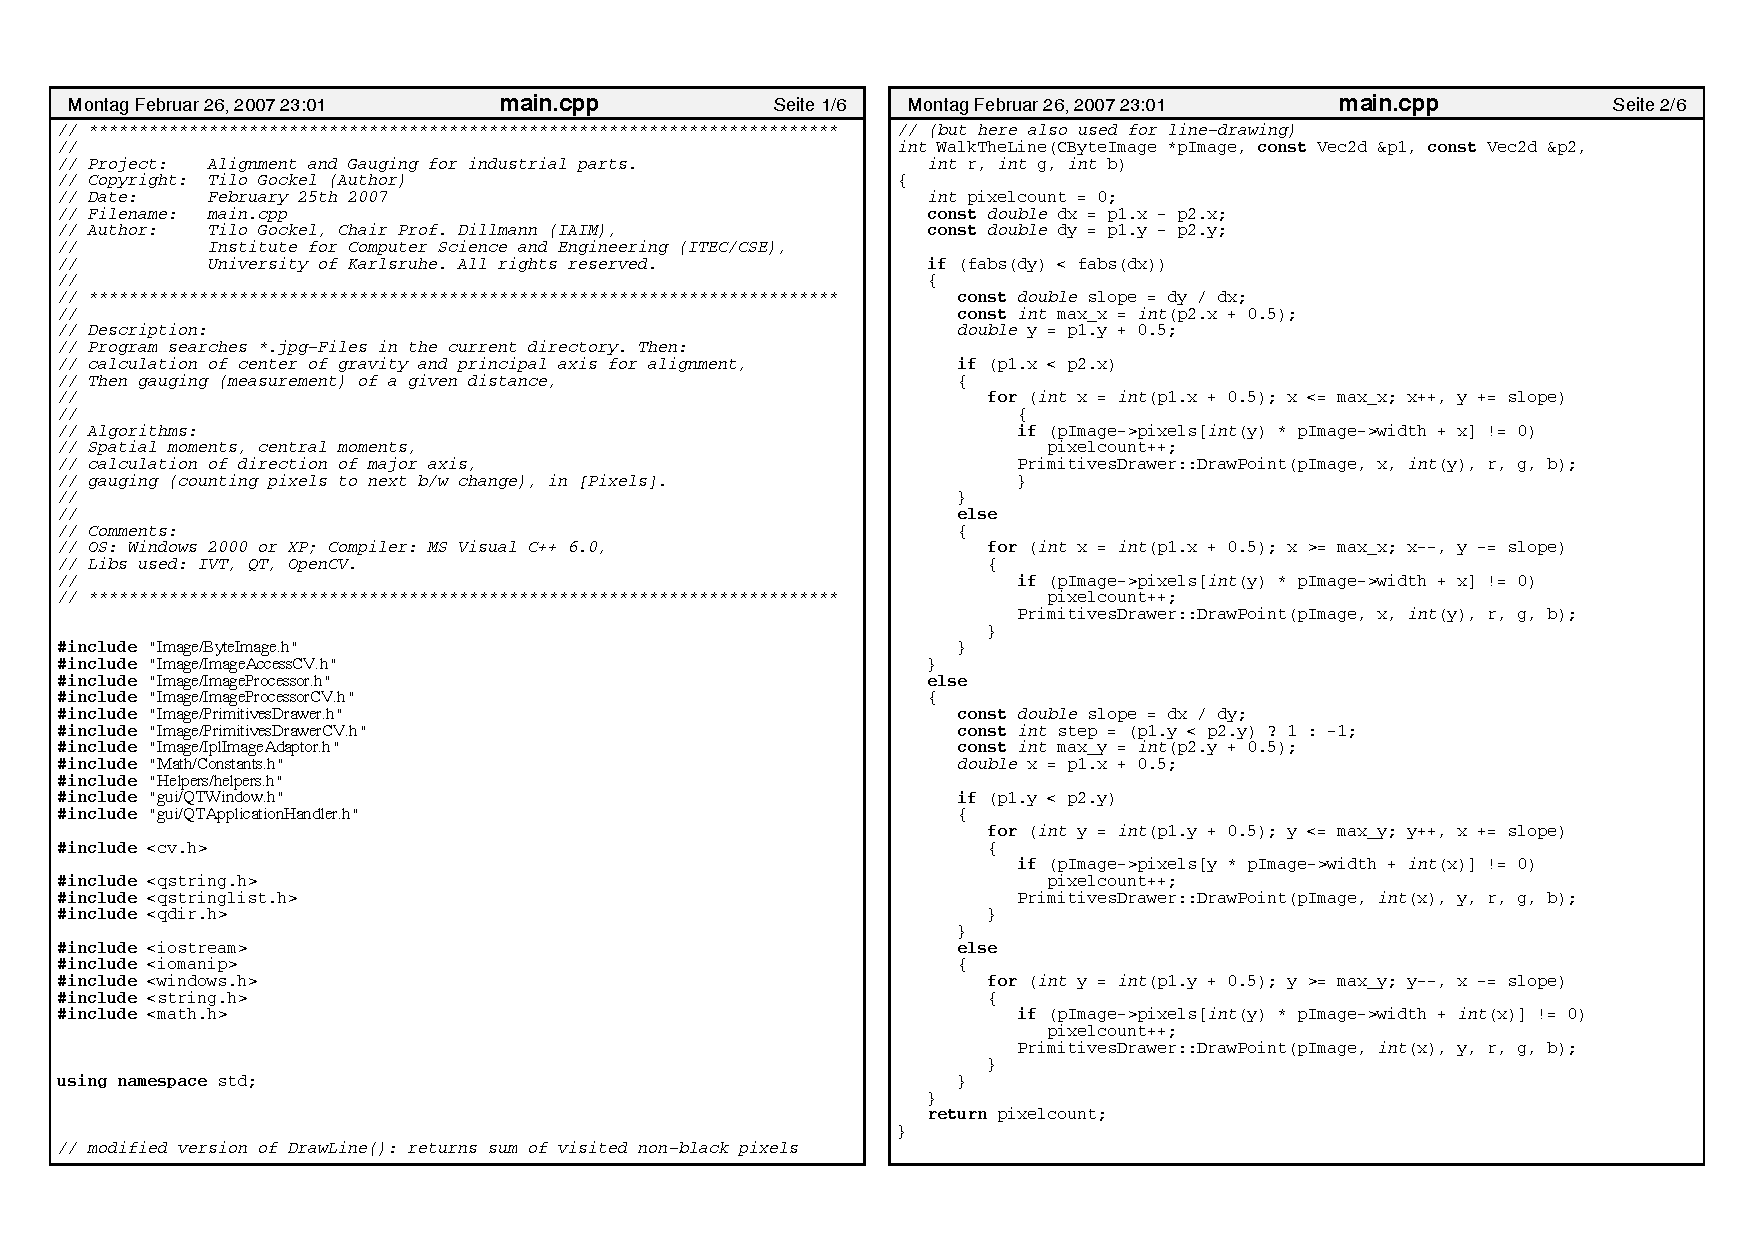
\includepdf[
 pages={-},
 nup=1x1,
 landscape=true,
 noautoscale=false,
 turn=false,
 scale=0.80,
 trim= 0mm 0mm 0mm 0mm,
 clip=true,
 pagecommand={},
 delta=0mm 0mm
]{BilderAnhangC/main_cpp.pdf}












                 % C
\chapter{Datenbl�tter}\index{Datenbl�tter}


\textcolor{darkred}{Anmerkung: Wenn das Thema der Diplomarbeit auch Hardware-Komponenten bzw. den Aufbau eines Demonstrators eingeschlossen hat, so ist ein Anhang mit den wichtigsten Datenbl�ttern sehr sinnvoll. Zum Einen k�nnen interessierte Leser direkt ohne Internetrecherche die Betriebsparameter der Komponenten einsehen, zum Anderen ist somit auch eine gute Dokumentation des Systems f�r die Bedienung durch andere Anwender als den Autor gegeben. Auch wenn die Datenbl�tter normalerweise online verf�gbar sind, so erspart der beigef�gter Anhang dem Anwender eine aufw�ndige Recherche. Die Anzahl Seiten sollte 25--30 nicht �berschreiten.}

\textcolor{darkred}{Genau wie bei den Quelltextabschnitten im Anhang muss aber auch bei den Datenbl�ttern ein kurzer Abschnitt vorweg geschickt werden, welcher die Auswahl der Datenbl�tter und die Relevanz erkl�rt.}

\textcolor{darkred}{Die einzuf�genden Datenbl�tter sollten im pdf-Dateiformat vorliegen und nicht als Grafik, sondern als ganze Seite einzuf�gen.}


Die nachfolgenden Datenbl�tter erl�utern Systemparameter, Funktionsweise, Anschlussvarianten und Betriebsarten zu dem im Rahmen der vorliegenden Arbeit verwendeten Maxon-Motorregler ADS\_E 50-10.



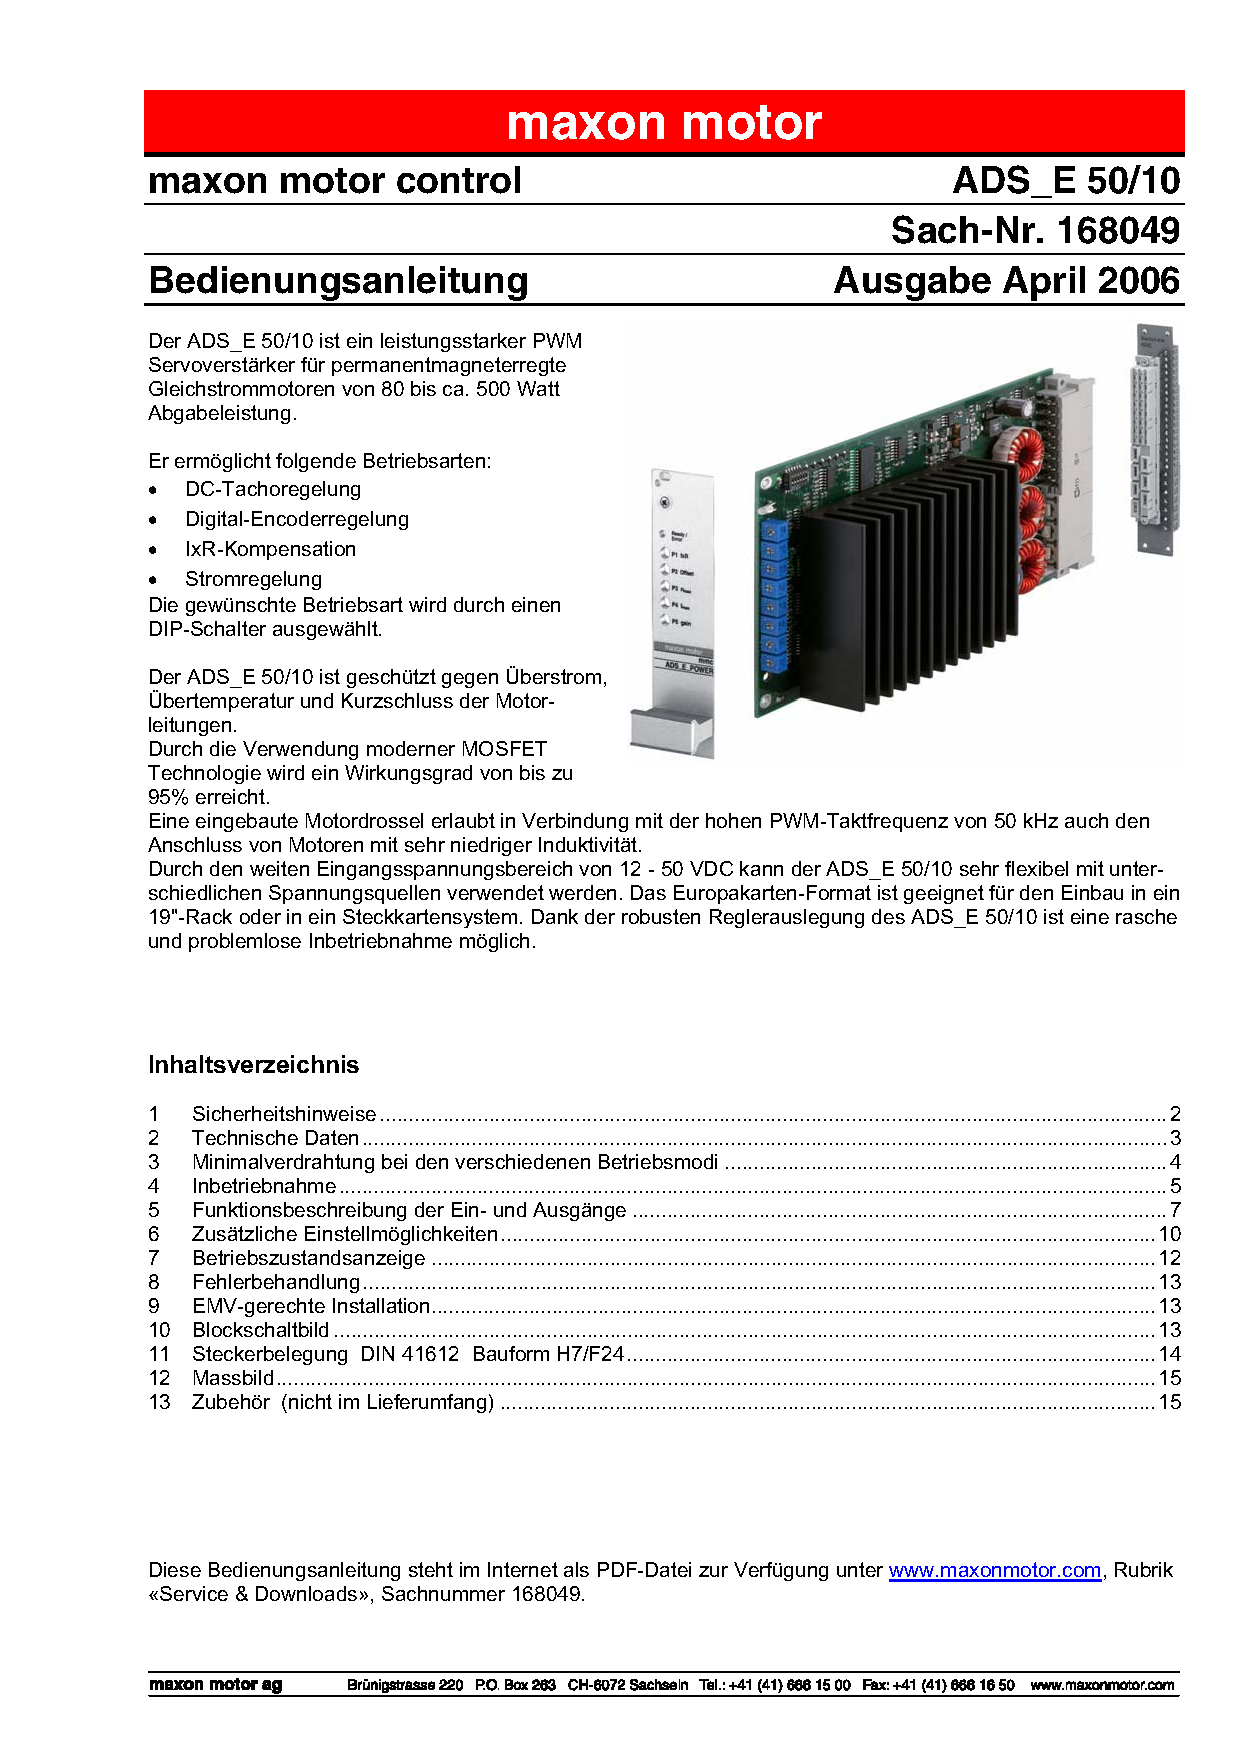
\includepdf[
   pages={-},
   nup=1x1,
   landscape=false,
   noautoscale=false,
   turn=false,
   scale=0.8,
   trim= 0mm 0mm 0mm 0mm,
   clip=true,
   pagecommand={},
   delta=0mm 0mm
]{BilderAnhangD/Seiten_aus_ads_e50_10_de.pdf}

%
% Vorsicht: Pfad- und Dateiname darf keine Leerzeichen enthalten
%

              % D
\chapter{Glossar}\index{Glossar}
\label{anhang_e}



\textcolor{darkred}{Anmerkung: Das vorliegende Glossar wurde ohne die Zuhilfenahme der speziellen Glossarumgebungen von Latex erstellt, um eine etwas freiere Formatierung nutzen zu k�nnen.}
\medskip



\interlinepenalty=10000 % keine Schusterjungen, keine Hurenkinder



\begin{description}

\item[\bf{2,5D-Datensatz}] $\rightarrow$Tiefenbild.

\item[\bf{3D-Modell, 3D-Modellerfassung (optische)}] Der Begriff des 3D-Modells wird in der vorliegenden Arbeit f�r wasserdichte Oberfl�chenmodelle verwendet. Dies dient zur Abgrenzung gegen�ber 3D-Volumenmodellen und $\rightarrow$Tiefenbildern. Der Begriff der Optischen 3D-Modellerfassung umschlie�t hier neben der eigentlichen Sensordatenauswertung auch die $\rightarrow$3D-Registrierung und die Schritte der Nachbearbeitung wie Gl�tten und Ausd�nnen der Daten und Stiching-Operationen.

\item[\bf{3D-Registrierung}] Vgl. Abschnitte 2.4, 4.3 und $\rightarrow$Registrierung.

\item[\bf{Aktive Musterprojektion}] Der Begriff der Aktiven Musterprojektion kennzeichnet Musterprojektionsverfahren, welche einen kalibrierten Musterprojektor voraussetzen. Vgl. entsprechend auch $\rightarrow$Passive Musterprojektion.

\item[\bf{Aktive Optische Verfahren}] Der Terminus Aktive Optische Verfahren kennzeichnet 3D-Datenerfassungsverfahren, welche eine zus�tzliche Lichtquelle voraussetzen. Dies ist auch bei dem Verfahren der durch $\rightarrow$Passive Musterprojektion erg�nzten Stereopsis der Fall, dennoch wurde in der Darstellung zur Klassifizierung dieses Verfahren naheliegenderweise als Sonderfall hinter der Standard-Stereopsis aufgef�hrt (Abbildung 2.1).

\item[\bf{Apertur, numerische}] Die numerische Apertur NA eines optischen Elementes, beispielsweise eines Objektivs, ist ein Ma� f�r seine Lichtst�rke bzw. sein Auf"-l�sungsverm�gen. Die NA ist proportional zum �ffnungswinkel: $NA = n \cdot \sin \frac{\alpha }{2}$, mit $n$: Brechzahl. Oft wird statt der NA auch der Begriff der Blendenzahl $F$ verwendet, hier besteht ein umgekehrt proportionaler Zusammenhang.

\item[\bf{A priori-Szenenwissen}] Liegen vor Beginn der 3D-Erfassung bereits Informationen zur Geometrie des zu erfassenden Objektes im Erfassungssystem vor, so spricht man von a priori-Szenenwissen. Dies kann beispielsweise die Kenntnis der maximalen Objektausdehnung in $z$-Richtung sein, hilfreich zur Beschr�nkung des Suchraumes bei der Korrespondenzfindung. Ein weiteres Beispiel ist die Kenntnis der Anordnung der Profillinien auf der Objektoberfl�che beim Lichtschnittverfahren; sie erm�glicht eine einfache und schnelle $\rightarrow$Vernetzung der $\rightarrow$Tiefenbilder.

\item[\bf{Bildaufnehmer}] Der allgemeine Begriff des Bildaufnehmers steht in der vorliegenden Arbeit f�r zweidimensionale optische Sensoren bzw. Matrixkameras mit CCD- oder CMOS-Sensor.

\item[\bf{Direkte Lineare Transformation, DLT}] $\rightarrow$Abschnitt 3.2.3.

\item[\bf{Disparit�t}] Bei dem Ansatz des $\rightarrow$Stereosehens versteht man unter der Disparit�t den durch den Abstand der beiden Bildaufnehmer zueinander entstehenden Versatz der Abbildungen eines Objektpunktes. Dieser Versatz ist abh�ngig von der Entfernung des Objektes und entsprechend kann hieraus auf die Entfernung r�ckgerechnet werden.

\item[\bf{Epipolargeometrie, Epipolarlinie, Epipol}] $\rightarrow$Abschnitt 3.2.5.

\item[\bf{Extrinsische Parameter}] Hiermit sind Position und Orientierung eines $\rightarrow$Bildaufnehmers im vorgegebenen Weltkoordinatensystem bezeichnet. Sie sind gemeinsam mit den $\rightarrow$intrinsischen Parametern aus der Kalibrierung erh�ltlich (vgl. Abschnitte 3.2 und 3.3.1).

\item[\bf{Fringe Pattern, Fringe Projection}] Der englische Begriff Fringe Pattern bzw. Fringe Projection (Fringe: dtsch. Rand, Saum) entspricht dem deutschen Begriff des Streifenmusters bzw. der Streifen-, Bin�r- oder Graycode-Projektion (vgl. Abschnitt 2.2.2).

\item[\bf{Geod�sie}] (Griech.: geo: Erde, dasei: teilen). Nach der klassischen Definition von F. R. Helmert ist die Geod�sie die \glqq Wissenschaft von der Ausmessung und Abbildung der Erdoberfl�che.\grqq\ Ein wichtiges Messprinzip der Geod�sie ist die $\rightarrow$ Triangulation.

\item[\bf{Homographie}] Eine Homographie bedeutet die lineare Abbildung bzw. projektive Transformation einer Ebene im dreidimensionalen Raum auf eine andere Ebene in Form einer 3$\times$3-Transformationsmatrix. Eine g�ngige Anwendung ist die Entzerrung projizierter Bilder. Hier wird die $\rightarrow$Rektifikation durch eine Homographie hergestellt.

\item[\bf{\emph{hsv}-Farbraum, \emph{hsv}-Modell}] Vgl. Rot-Gr�n-Blau-Farbraum, hier stellen die drei Werte nicht die drei Grundfarben dar, sondern stehen f�r \emph{hue} (Farbwert), \emph{saturation} (S�ttigung) und \emph{value} (Helligkeit). Die Umwandlung zwischen \emph{rgb} und \emph{hsv} ist m�glich, allerdings nicht immer eindeutig (vgl. Abschnitt 2.2.4).

\item[\bf{Intraoral}] Im Mundraum.

\item[\bf{Intrinsische Parameter}] Hiermit sind Kenngr��en wie Brennweite $f$ des Objektivs, Pixelgr��e des Bildaufnehmers in $x$ und $y$, Bildursprung (Position des Bildursprungs relativ zum Kamerakoordinatensystem) und Objektivverzeichnungen eines Bildaufnehmers mit zugeh�riger Optik bezeichnet. Zusammen mit den $\rightarrow$extrinsischen Parametern sind sie erh�ltlich aus der Kalibrierung (vgl. Abschnitte 3.2 und 3.3.1).

\item[\bf{Kondensor, Kondensorlinse}] Ein Kondensor ist ein optisches System aus einer oder mehreren Sammellinsen oder Spiegelfl�chen zwischen Lichtquelle und abzubildendem Objekt (Dia beim Projektor, Objekttr�ger beim Mikroskop). Der Kondensor lenkt das Licht, welches das Objekt durchsetzt, in das abbildende Objektiv. Kondensorlinsen sind oft asph�risch ausgeformt, um eine m�glichst kurze Brennweite und damit eine m�glichst kleine Bauform des Ger�tes zu erm�glichen.

\item[\bf{Korrespondenzproblem, Korrespondenzanalyse}] Vgl. Abschnitt 2.2.1.

\item[\bf{Lichtschnitt}] $\rightarrow$Linienlaser.

\item[\bf{Linienlaser}] Er stellt einen um eine Zylinder- bzw. Powell-Linse erweiterten Punktlaser dar. Der Laserstrahl wird hierdurch f�cherf�rmig aufgeweitet und kann somit auf einer Projektionsfl�che als gut erkennbare Laserlinie abgebildet werden. Anwendung findet der Linienlaser h�ufig in triangulationsbasierenden Laserscannern, das Verfahren wird dann als Lichtschnittverfahren bezeichnet.  Das Verfahren ist bis auf die einfachere Korrespondenzauf"-l�sung identisch mit der zeitlich codierten Musterprojektion (Bin�re M., Graycode-M., vgl. 2.2.1), dennoch wird im Sprachgebrauch unterschieden. Diese Verfahren werden meist als \emph{auf strukturiertem Licht basierend} bezeichnet.


\item[\bf{Matching}] Wird der Begriff des Matchings wie in der vorliegenden Arbeit auf Oberfl�chendatens�tze ($\rightarrow$Tiefenbilder) angewandt, so kennzeichnet er die Bestimmung der Transformation, um die Datens�tze in ein gemeinsames Koordinatensystem zu �berf�hren. Er ist gleichbedeutend mit dem Begriff der $\rightarrow$3D-Registrierung.

\item[\bf{Merging}] Der Begriff des Merging wird in der vorliegenden Arbeit f�r den Vorgang der Eingliederung eines bereits registrierten, vorvernetzten  $\rightarrow$2,5D-Datensatzes in einen bestehenden 3D-Datensatz auf dem Weg zur Erstellung eines geschlossenen $\rightarrow$3D-Modells verwendet. Hierzu ist zumindest teilweise eine Neuvernetzung erforderlich (zur Vorgehensweise und zu Problemen hierbei vgl. beispielsweise [V�lzow 03]).

\item[\bf{Meshing}] $\rightarrow$Vernetzung.

\item[\bf{One-Shot-Verfahren}] Der Begriff kennzeichnet musterprojektionsbasierte Verfahren zur optischen 3D-Datenakquisition, bei welchen ein einziges aufgenommenes Bild ausreicht, um ein $\rightarrow$Tiefenbild zu erstellen. Der Begriff wurde von Marc Proesmans gepr�gt [Proesmans 96a].

\item[\bf{Passive Musterprojektion}]  Im Gegensatz zu dem Verfahren der $\rightarrow$Aktiven Musterprojektion kommen hier zwei oder mehr kalibrierte Kameras, erg�nzt durch einen Musterprojektor, zum Einsatz ($\rightarrow$Stereopsis). Dieser ist nicht kalibriert, sondern dient nur dazu, die Szene zu aktivieren bzw. der Szene neue Merkmale zuzuordnen, um dieserart die Korrespondenzfindung zu erleichtern.

\item[\bf{Phasenschiebeverfahren, Phase Shifting}] Vgl. Abschnitt 2.2.3

\item[\bf{Punktwolke}] Mit dem Begriff der Punktwolke wird in der vorliegenden Arbeit allgemein ein nicht $\rightarrow$vernetzter $\rightarrow$2,5D-Datensatz oder 3D-Datensatz bezeichnet. �quivalent ist im Englischen der Begriff \emph{Point Cloud} bzw. -- spezifisch im unorganisierten Fall -- \emph{Scattered Point Data}.

\item[\bf{Region Growing, Regionenwachstum}] Das Region Growing-Verfahren ist ein regionenbasiertes Segmentierungsverfahren. Bei diesem Verfahren wachsen homogene Regionen ausgehend von vorgegebenen Saatpunkten. Zu einer dieserart entstehenden Region werden angrenzende Bildpunkte hinzugenommen, solange ein vorgegebenes Homogenit�tskriterium erf�llt ist (typisches Kriterium: Schwellwert f�r die Grauwertdifferenz).

\item[\bf{Registrierung}] Der Begriff der Registrierung wird in der vorliegenden Arbeit als Kurzform f�r $\rightarrow$3D-Registrierung verwendet. Dies dient der Abgrenzung gegen�ber der anders lautenden Definition der Registrierung in der (medizinischen) Bildverarbeitung. Hier wird der Begriff f�r die Zuordnung von 2D-Bildinformationen zueinander gebraucht (monomodal: Bsp. radiologische Daten, multimodal: Bsp. radiologische Daten zu Ultraschalldaten).

\item[\bf{Rektifikation}] Unter Rektifikation versteht man den Vorgang, die Bildebenen zweier Kameras, die in der Realit�t nicht in der gleichen Ebene liegen, sondern verschoben und/oder gegeneinander rotiert sind, auf eine gemeinsame virtuelle Bildebene abzubilden, in welcher dann die jeweiligen  Epipolarlinien kollinear zueinander und zu den Basisvektoren verlaufen.
Ein Vorteil, der hieraus entsteht, ist die M�glichkeit der Anwendung einfacherer und schnellerer Korrelationsverfahren. Die Rektifikation wird durch eine $\rightarrow$Homographie hergestellt (vgl. auch [Trucco 98,7.3.7]).

\item[\bf{Running Sum}] $\rightarrow$Sum Table

\item[\bf{Sch�rfentiefe}] Mit Sch�rfentiefe wird die Ausdehnung des scharf abgebildeten Bereiches entlang der optischen Achse eines optischen Systems bezeichnet (auch: Abbildungstiefe, umgangssprachlich oft auch: $\rightarrow$Tiefensch�rfe). Zur rechnerischen Bestimmung wird f�r den Zerstreuungskreis auf dem $\rightarrow$Bildaufnehmer ein maximaler Durchmesser vorgegeben (vgl. auch [Schr�der 77]).

\item[\bf{Splatting}] Ein Problem bei der Visualisierung von 3D-Oberfl�chendaten ist die Notwendigkeit der zeitaufw�ndigen $\rightarrow$Vernetzung. Neue Verfahren zur Visualisierung von 3D-Daten setzen keine Nachbarschaftsbeziehungen zwischen den Punkten voraus, sondern dehnen im Moment des Renderings bzw. der Anzeige der Daten durch Projektion auf eine Fl�che (Bildschirm) einzelne den Punkten zugewiesene Elementfunktionen so weit aus, dass sich der visuelle Eindruck einer geschlossenen Fl�che ergibt. Man unterscheidet hierbei Surface Splatting und Volume Splatting (vgl. auch QSplat, [Rusinkiewicz 00]).

\item[\bf{Stereopsis, Stereosehen}] Unter dem Begriff Stereopsis versteht man den Vorgang der visuellen Wahrnehmung der Tiefe oder Entfernung von Objekten. Der Begriff leitet sich ab aus den griechischen Worten \emph{Stereo} f�r r�umlich und \emph{Opsis} f�r Sehen oder Sicht. Die Tiefeninformation wird hierbei gewonnen aus dem entfernungsabh�ngigen Versatz der Bildinformationen zwischen den zwei Augen oder Bildaufnehmern.

\item[\bf{Sum Table}] Der Begriff Sum Table bezeichnet die Ablage einer fortlaufend gebildeten Summe (Running Sum) in einer n-dimensionalen Tabelle. Bsp. (1D):
$S_{\sum {x_k } }  = [\sum\limits_1 {x_k ,} \sum\limits_2 {x_k ,} ...,\sum\limits_n {x_k }]$. Teilsumme $\sum\limits_{k = l}^m {x_k }$ kann hiermit nun schnell gebildet werden. F�r den zweidimensionalen Fall vgl. Abschnitt 3.4.2: Optimierte ZNCC.

\item[\bf{Tiefenbild}] Mit dem Begriff Tiefenbild wird eine Darstellungsform f�r H�heninformationen bezeichnet, welche in einem Grauwertbild mit den Bildpunktkoordinaten $x,y$ diesen auch einen $z$-Wert in Form ihres Grauwertes zuordnet. Die Darstellungsform kann leicht umgewandelt werden in eine $\rightarrow$3D-Punktwolke, deren Punkte alle eindeutig in die $xy$-Ebene projizierbar sind (man spricht dann von 2,5D-Datensatz). Ein Tiefenbild kann somit kein geschlossenes $\rightarrow$3D-Modell darstellen, sondern nur eine Sicht auf ein Objekt vermitteln. Seltener auch: Tiefenkarte.

\item[\bf{Tiefensch�rfe}] $\rightarrow$Sch�rfentiefe.

\item[\bf{Transluzenz}] Die Transluzenz bezeichnet die Eigenschaft eines Objektes, teilweise lichtdurchl�ssig zu sein. In Abgrenzung zur Transparenz kann man Transluzenz als Lichtdurchl�ssigkeit beschreiben und Transparenz als Bilddurchl�ssigkeit.

\item[\bf{Triangulation}] Der Begriff der Triangulation wird in der vorliegenden Arbeit zweifach verwendet. Zum einen bezeichnet er den Vorgang der Vernetzung einer $\rightarrow$Punktwolke zu einem Dreiecksnetz (Bsp.: Delaunay-Triangulation, Abschnitt 4.5.1), zum anderen die Berechnung der Tiefe auf Basis von Dreiecksbeziehungen bei der optischen 3D-Datenerfassung (vgl. Abbildung E.1 und Abschnitt 3.2.4).
%
\begin{figure}[H]
\centering
   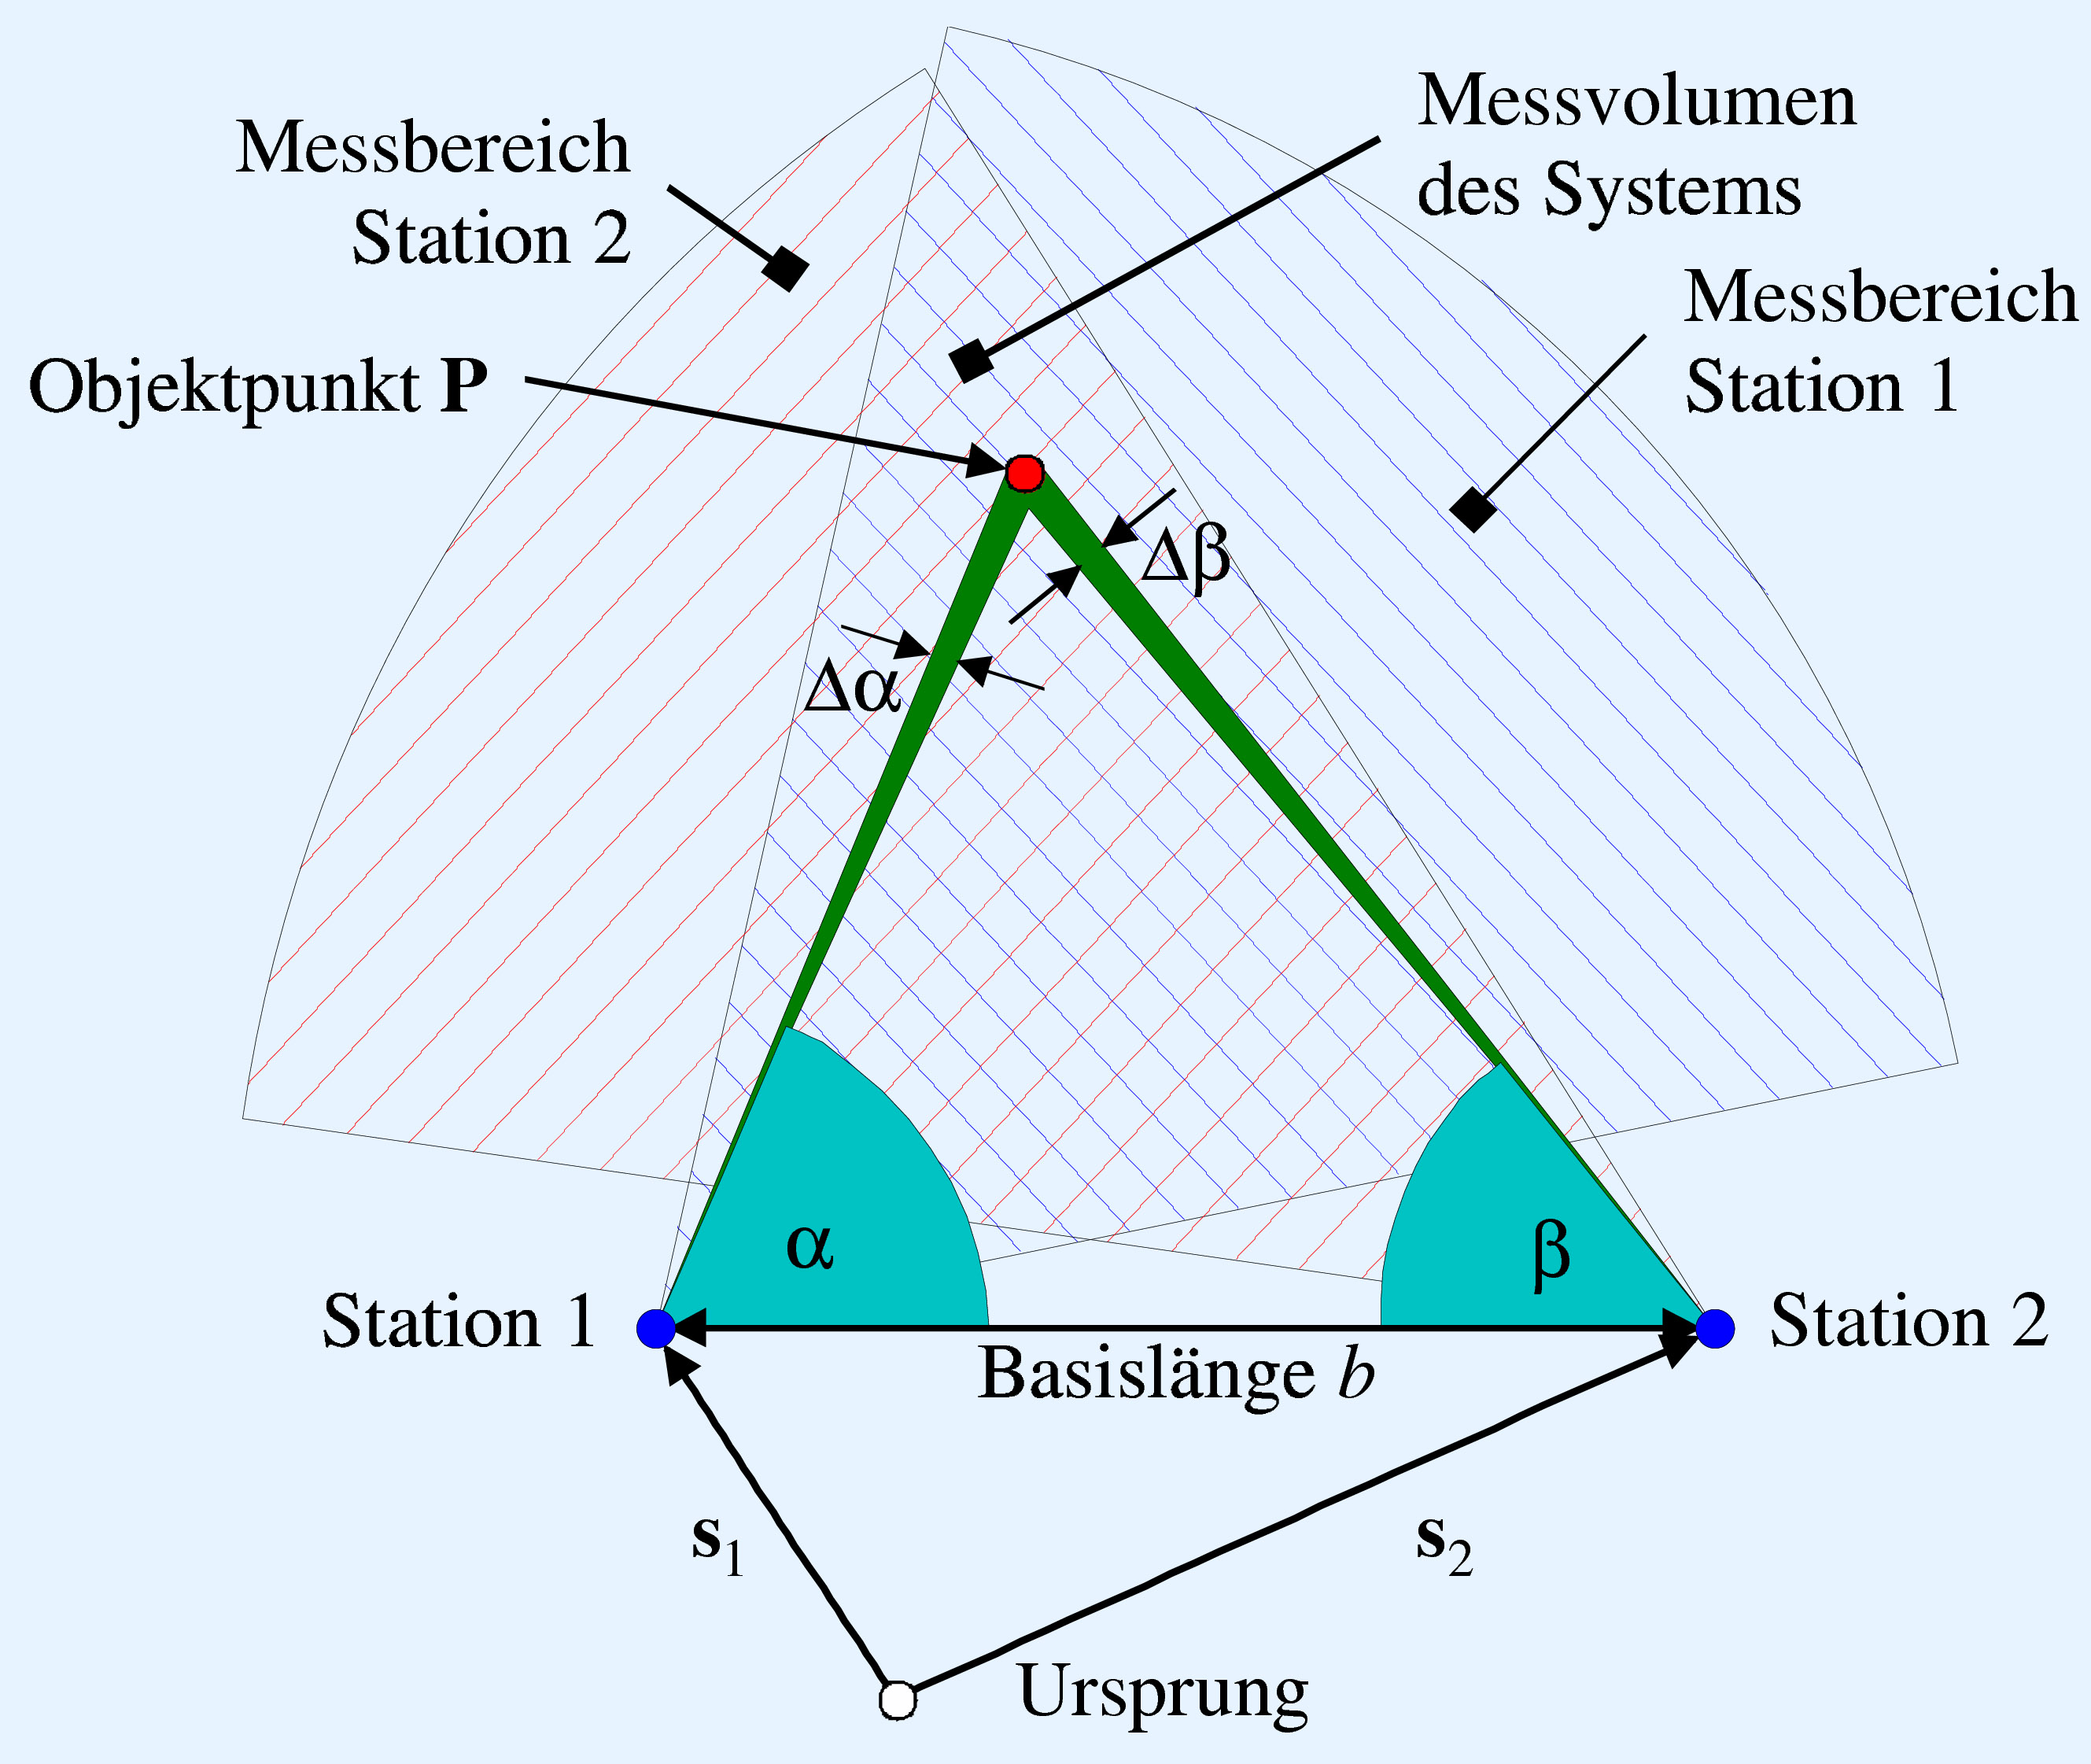
\includegraphics[scale=0.55]{BilderAnhangE/Triangulation2d.jpg}
   \caption{Triangulation (Bildquelle: [Wikipedia 07]).}
   \label{AnhangE_Triangulation}
\end{figure}
%
\glqq (\dots) Von zwei verschiedenen Stationen an den Positionen $\bf{s_1}$ und $\bf{s_2}$ wird der zu bestimmende Zielpunkt $\bf{P}$ angepeilt. Dabei erh�lt man die beiden Winkel $\alpha$ und $\beta$ mit der Genauigkeit $\Delta \alpha$ und $\Delta \beta$. Unter Kenntnis der Basisl�nge $b$ kann man dann die Koordinaten von $\bf{P}$ relativ zum Koordinatenursprung bestimmen.\grqq\ (Zitat aus: [Wikipedia 06]). Ein bekanntes optisches Winkelmessger�t der $\rightarrow$Geod�sie ist der Theodolit.
%
\item[\bf{Vernetzung}] Mit dem Begriff der Vernetzung wird die Erstellung einer Oberfl�che aus einer Punktwolke durch Einf�gen von Kanten zwischen den Punkten bezeichnet. Im allgemeinen Fall entstehen hieraus $n$-Ecke, im speziellen Fall Dreiecke ($\rightarrow$Triangulation).
%
\item[\bf{Weltkoordinatensystem}] Der Begriff Weltkoordinatensystem ist in der vorliegenden Arbeit anders belegt als in der klassischen Geod�sie: Gemeint ist ein dreidimensionales kartesisches Koordinatensystem, in welchem die Daten in der Einheit [Meter] bzw. [Millimeter] eingetragen sind,
welches aber nicht in Bezug steht zu geographischen Landeskoordinaten.
\end{description}
\interlinepenalty=100



                    % E
\end{appendix}



% Erstes Literaturverzeichnis, ohne BibTeX

\interlinepenalty=10000 % Literatureintr�ge: Abs�tze zusammenhalten
\cleardoublepage
\addcontentsline{toc}{chapter}{Literatur}   
%F�r das nachfolgende exemplarische Literaturverzeichnis wurde die einfache thebibliography-Umgebung von Latex verwendet. F�r Studien- und Diplomarbeiten mit weniger als 40 Quellen sollte diese auf jeden Fall ausreichen und hat gegen�ber dem komplexen Bibtex-Paket weiterhin den Vorteil flexiblerer Formatierungsm�glichkeiten.
%
%Im Anschluss an das exemplarische Literaturverzeichnis ist ein zweites Verzeichnis beigef�gt, welches weiterf�hrende Quellen zum vorliegenden Latex-Template enth�lt: Download-Links zur Software, freie Online-Latex-Handb�cher usw.



\begin{thebibliography}{Ti}



\bibitem[Abdel-Aziz 71]{abdelaziz71} Y. I. Abdel-Aziz and H. M. Karara, \glqq Direct linear transformation from comparator coordinates into object space coordinates in close-range photogrammetry\grqq, in: Symposium on Close-Range Photogrammetry, issue 11, pp. 1--18, University of Illinois at Urbana-Champaign, 1971.

\bibitem[AutTech 07]{auttech07} Firma Automation Technology GmbH in 22946 Trittau, Produkt�bersicht, Downloads und Datenbl�tter.  URL: \url{http://www.automationtechnology.de}

\bibitem[Dang 06]{dang06} T. Dang, C. Stiller and C. Hoffmann, \glqq Self-calibration for Active Automotive
Stereo Vision\grqq, Proc. of the IEEE Intelligent Vehicles Symposium, pp. 364--369, Japan, Tokyo, 2006.

\bibitem[Fisher 96]{fisher96} R. B. Fisher and D. K. Naidu. \glqq A Comparison of Algorithms for Subpixel Peak Detection\grqq\, in: Advances in Image Processing, Multimedia and Machine Vision, Springer-Verlag, Heidelberg, 1996. Online erh�ltlich via CiteSeer.

\bibitem[Gamma 04]{gamma04} E. Gamma, D. Riehle u.\,a., \glqq Entwurfsmuster -- Elemente wiederverwendbarer objektorientierter Software\grqq, Addison-Wesley-Verlag, M�nchen, 2004.

\bibitem[G�hring 02]{guehring02} J. G�hring, \glqq 3D-Erfassung und Objektrekonstruktion mittels Streifenprojektion\grqq, Dissertation, Universit�t Stuttgart, Institut f�r Photogrammetrie, 2002. Online erh�ltlich via URL: \url{http://elib.uni-stuttgart.de/opus/volltexte/2006/2715/pdf/Guehring_diss.pdf}

\bibitem[Hoppe 02]{hoppe02} H. Hoppe, C. K�bler, J. Raczkowsky und H. W�rn, \glqq Ein neues und leicht zu implementierendes
Modell zur pr�zisen Kalibration von Kameras und Videoprojektoren\grqq, in: Medicine Meets Virtual Reality (MMVR 02), pp. 229--232, Newport Beach, USA, 2002.

\bibitem[Huckle 02]{huckle02} T. Huckle und S. Schneider, \glqq Numerik f�r Informatiker\grqq, Springer-Verlag, Heidelberg, 2002.

\bibitem[K�ferstein 98]{kaeferstein98} B. K�ferstein, \glqq 3D-Verformungsmessungen auf 10nm genau -- Grundlagen und Anwendungen der Speckle-Interferometrie\grqq, Institutsmittelung Nr. 23, Institut f�r Maschinenwesen (IMW), Technische Universit�t Clausthal, 1998.

\bibitem[Kitware 07]{kitware07} Firma Kitware Inc. (USA), Online-Produktpr�sentation und freier Download der Software-Bibliothek VTK -- Visualization Toolkit. URL: \url{http://www.kitware.com}

\bibitem[Luhmann 03]{luhmann03} T. Luhmann, \glqq Nahbereichsphotogrammetrie: Grundlagen -- Methoden -- Anwendungen\grqq, Wichmann-Verlag, Heidelberg, 2003.

\bibitem [Marqu 63]{marqu63} D. Marquardt, \glqq An Algorithm for Least-Squares Estimation of Nonlinear Parameters\grqq, SIAM J. Appl. Math., vol. 11, pp. 431--441, 1963.

\bibitem[Pentax 07]{pentax07} Firma Pentax, Online-Produktspektrum und Datenbl�tter. URL: \url{http://www.pentax.de}

\bibitem[Pollefeys 03]{pollefeys03} M. Pollefeys, L. Van Gool u.a., \glqq3D Capture of Archaeology and Architecture with a Hand-Held Camera\grqq, Proc. of the ISPRS workshop on Vision Techniques for Digital Architectural and Archaeological Archives, Ancona, Italy, The Int. Archive of the Photogrammetry, Remote Sensing and Spatial Information Sciences, Vol. XXXIV, Part 5/W12, pp. 262--267, July 2003.

\bibitem[SAC 07]{sac07} Firma SAC GmbH in 76149 Karlsruhe, Online-Produktspektrum und Datenbl�tter. URL: \url{http://www.sac-vision.de}.

\bibitem[SuK 07]{suk07} Firma Sch�fter und Kirchhoff GmbH in 22525 Hamburg,
Online-Produktspektrum, bes. interessant: die Applikationsschriften. URL:
\url{http://www.sukhamburg.de}

\bibitem[TI 07]{ti07} Firma Texas Instruments, Online-Produktspektrum, Datenbl�tter und Downloads. URL: \url{http://www.ti.com}

\bibitem[TIS 07]{tis07} Firma The\,Imaging\,Source Europe GmbH in 28215 Bremen, Produkt�bersicht, Downloads und Datenbl�tter. URL: \url{http://www.theimagingsource.com}


\bibitem[Trolltech 07]{trolltech07} Fa. Trolltech Inc., Produktinformationen und Download zur Software-Bibliothek Qt. URL: \url{http://www.trolltech.com}

\bibitem[Trucco 98]{trucco98} E. Trucco and A. Verri, \glqq Introductory Techniques for 3-D Computer Vision\grqq, Verlag Prentice\,Hall, 1998.

\bibitem[VC 07]{vc07} Firma Vision Components in 76275 Ettlingen, Online-Produkt�bersicht, Datenbl�tter und Tutorials , URL: \url{http://www.vision-components.com}

\bibitem[Vuylsteke 90]{vuylsteke90} P. Vuylsteke and A. Oosterlinck, \glqq Range image acquisition with a single binary-encoded light pattern\grqq, Tagungsband: IEEE Transactions on Pattern Analysis and Machine Intelligence (PAMI), Vol.\,12, No.\,2, pp.\,148--164, 1990.

\bibitem[W�rn 05]{woern05} H. W�rn und U. Brinkschulte, \glqq Echtzeitsysteme\grqq, Springer-Verlag, Heidelberg, 2005.

\bibitem[Zhang 00]{zhang00} Z. Zhang, \glqq Flexible camera calibration by viewing a plane from unknown orientations\grqq, IEEE Transactions on Pattern Analysis and Machine Intelligence (PAMI), Vol.\,22, No.\,11, pp.\,1330--1334, 2000, URL: <ftp://ftp.research.microsoft.com/pub/tr/tr-98-71.pdf> (31.05.2007).

\end{thebibliography}






% Zweites Literaturverzeichnis, mit BibTeX

\renewcommand\bibname{Weiterf�hrende Literatur zu wissenschaftlichen Ausarbeitungen}
\nocite{*} % auch die nicht verwendeten bibtex-Eintr�ge einblenden
\cleardoublepage
\addcontentsline{toc}{chapter}{Weiterf�hrende Literatur zu wissenschaftlichen Ausarbeitungen}
\bibliography{bibliografie}
\interlinepenalty=100



% Sachverzeichnis einf�gen

\renewcommand\indexname{Sachverzeichnis}
\cleardoublepage
\addcontentsline{toc}{chapter}{Sachverzeichnis}
\linespread{0.99} % Abhilfe zu Schusterjungen .. im Index. Die Zahl ist entspr zu variieren
\printindex                                 



% Schmutzblatt (leere Seite am Ende)

\newpage                                    
\pagestyle{empty}
\begin{figure}[H]
\centering

\includegraphics[width=0.9\textwidth]{BilderAllgemein/leer.jpg}
\end{figure}



\end{document}




















%
